\chapter{Thiết kế giao diện hệ thống}
\textit{Chương này trình bày thiết kế wireframe cho các màn hình chính của nền tảng luyện thi IELTS và TOEIC tích hợp AI. Nội dung tập trung mô tả vai trò của từng giao diện, cách tổ chức bố cục, luồng tương tác của người dùng và ý nghĩa của các thành phần trực quan trong việc hỗ trợ học tập, làm bài kiểm tra và quản trị hệ thống.}

\noindent\textit{\textbf{Ghi chú:} Toàn bộ hình ảnh giao diện trong chương này là ảnh chụp màn hình (screenshot) từ hệ thống thực tế do nhóm tác giả phát triển.}

\section{Thiết kế Wireframe}
Phần này mô tả tổng quan thiết kế wireframe của hệ thống trước khi triển khai giao diện hoàn chỉnh. Các wireframe được xây dựng nhằm xác định cấu trúc thông tin, vị trí các thành phần tương tác, luồng điều hướng chính và cách người dùng tiếp cận các chức năng cốt lõi. Thông qua việc chuẩn hóa bố cục cho từng nhóm màn hình như trang giới thiệu, xác thực, bảng điều khiển, khu vực làm bài, học với flashcard, hồ sơ cá nhân, blog và trang quản trị, nhóm phát triển có thể đảm bảo tính nhất quán trong trải nghiệm người dùng cũng như tạo nền tảng thuận lợi cho giai đoạn hiện thực giao diện sau này.

\subsection{Trang chủ}

\begin{figure}[H]
    \centering
    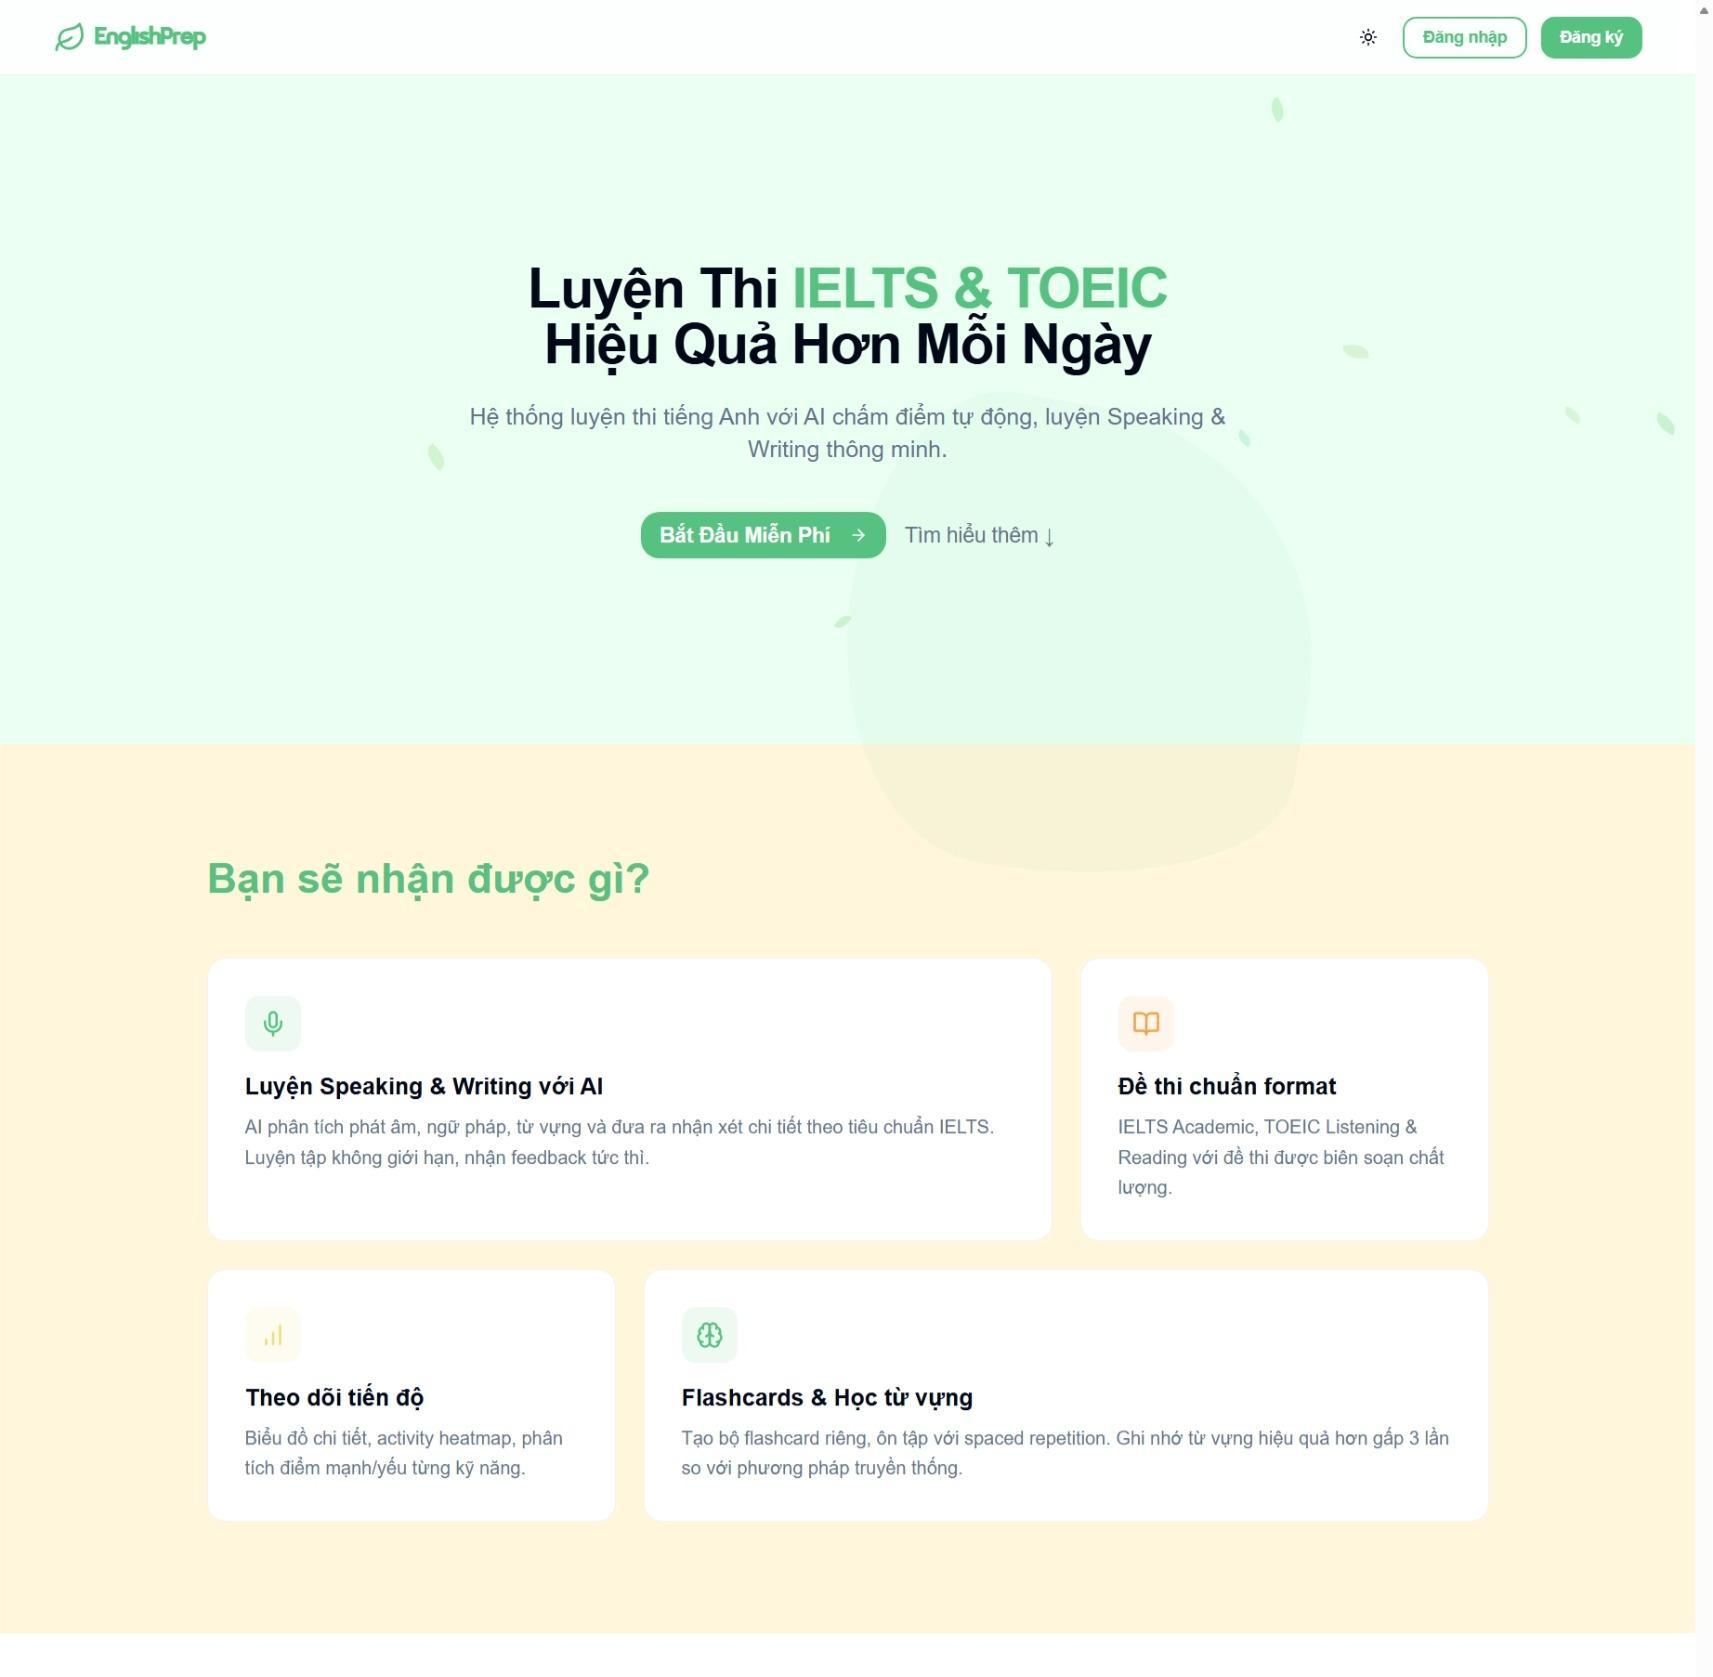
\includegraphics[width=0.75\linewidth]{graphics/ui/homepage.jpg}
    \captionsetup{skip=5pt}
    \caption{Giao diện trang chủ}
\end{figure}
\noindent Trang chủ là nơi người dùng nhìn thấy đầu tiên khi truy cập vào hệ thống. Phần đầu trang có logo và các nút ``Đăng nhập'', ``Đăng ký'' để người dùng bắt đầu nhanh. Ở giữa màn hình là tiêu đề chính, đoạn giới thiệu ngắn và hai nút hành động để dùng thử hoặc tìm hiểu thêm. Bên dưới là phần tóm tắt các lợi ích nổi bật của nền tảng như luyện Speaking và Writing với AI, làm đề theo chuẩn, theo dõi tiến độ và học bằng flashcard. Cách trình bày này giúp trang chủ dễ nhìn, dễ hiểu và tạo được ấn tượng rõ ràng ngay từ đầu.

\subsection{Trang xác thực}

\begin{figure}[H]
    \centering
    
\includegraphics[width=0.75\linewidth]{graphics/ui/auth.jpg}
    \captionsetup{skip=5pt}
    \caption{Trang xác thực người dùng}
    \label{h8}
\end{figure}
\noindent Trang xác thực được chia làm hai phần rõ ràng. Bên trái là khu vực giới thiệu với tiêu đề lớn, đoạn mô tả ngắn và các hình minh họa để tạo ấn tượng ban đầu. Bên phải là khối đăng nhập gồm logo, lời chào quay lại, ô nhập email, mật khẩu, nút ``Đăng nhập vào hệ thống'' và liên kết ``Đăng ký ngay''. Cách bố trí này giúp người dùng vừa nhận diện thương hiệu, vừa thao tác đăng nhập nhanh và dễ hiểu.



\subsection{Tính năng cho người học}

\subsubsection{Bảng điều khiển}

\begin{figure}[H]
    \centering
    
\includegraphics[width=0.75\linewidth]{graphics/ui/dashboard.jpg}
    \captionsetup{skip=5pt}
    \caption{Bảng điều khiển người dùng}
    \label{h9}
\end{figure}
\noindent Dashboard là màn hình chính sau khi người dùng đăng nhập. Giao diện được chia thành hai phần: thanh menu bên trái và khu vực nội dung ở bên phải. Menu bên trái giúp người dùng truy cập nhanh đến các chức năng như chọn đề thi, flashcards, luyện nói, tiến độ, lịch sử, blog, phòng chat và thông báo, đồng thời hiển thị thông tin tài khoản và nút đăng xuất. Ở phần nội dung chính, hệ thống hiển thị lời chào, nút ``Làm bài tập ngay'' và các thẻ thống kê như số đề đã làm, điểm trung bình, số bài đang thực hiện và số đề hiện có. Bên dưới là mục ``Hoạt động luyện tập'' với biểu đồ nhiệt, giúp người học theo dõi tần suất ôn luyện của mình một cách trực quan và dễ hiểu.

\subsubsection{Bài thi}


\begin{figure}[H]
    \centering
    
\includegraphics[width=0.75\linewidth]{graphics/ui/exam/exam-selection.jpg}
    \captionsetup{skip=5pt}
    \caption{Giao diện lựa chọn bài thi}
    \label{h10}
\end{figure}

\noindent Trang lựa chọn bài thi giúp người dùng tìm và chọn đề luyện tập một cách nhanh chóng. Ở phía trên có tab chuyển giữa IELTS và TOEIC, bên dưới là phần giới thiệu ngắn về kỳ thi đang được chọn. Các đề thi được hiển thị dưới dạng thẻ, mỗi thẻ cho biết tên bài, mức độ, một vài thông tin cơ bản và nút ``Vào thi ngay''. Cách trình bày này giúp người học dễ nhìn, dễ so sánh và chọn đúng bài mình muốn luyện.

\begin{figure}[H]
    \centering
    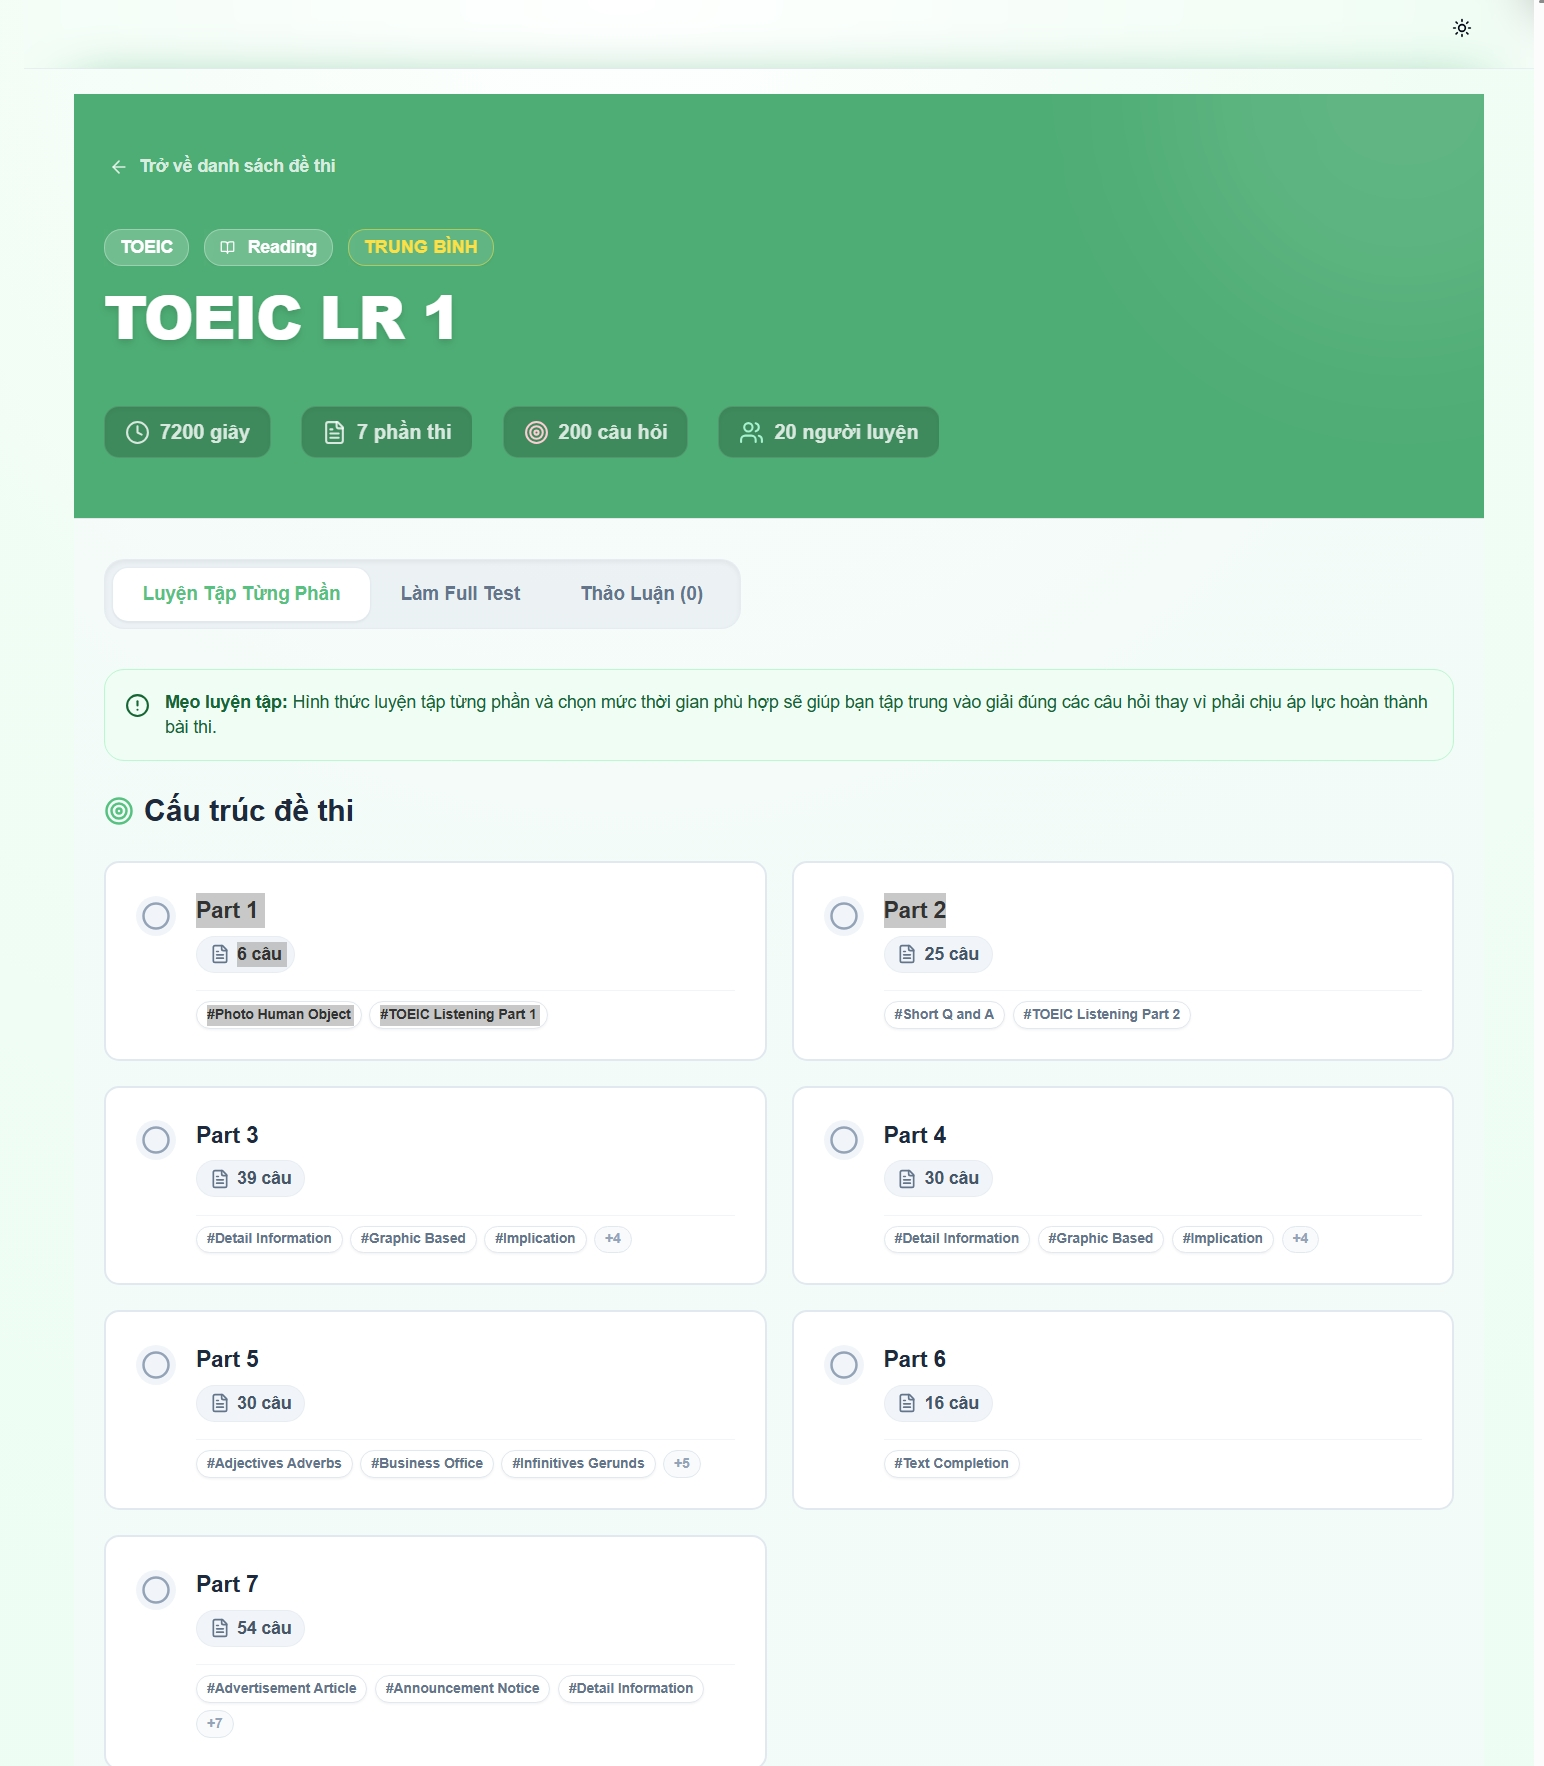
\includegraphics[width=0.75\linewidth]{graphics/ui/exam/exam-detail.jpg}
    \captionsetup{skip=5pt}
    \caption{Giao diện chi tiết bài thi}
    \label{h11}
\end{figure}
\noindent Trang chi tiết bài thi trình bày đầy đủ thông tin và các tùy chọn cấu hình trước khi người dùng bắt đầu làm bài. Bố cục sạch và rõ ràng giúp làm nổi bật các thông số như thời lượng, số lượng câu hỏi và mức độ khó, đồng thời cho phép lựa chọn chế độ làm bài có bấm giờ hoặc không bấm giờ. Người dùng có thể bắt đầu toàn bộ đề thi ngay lập tức hoặc chọn từng phần cụ thể để luyện tập theo nhu cầu. Bên cạnh đó, khu vực thảo luận và đánh giá còn hỗ trợ người học tham khảo nhận xét từ cộng đồng để hình dung trước chất lượng và độ thử thách của bài thi.

\begin{figure}[H]
    \centering
    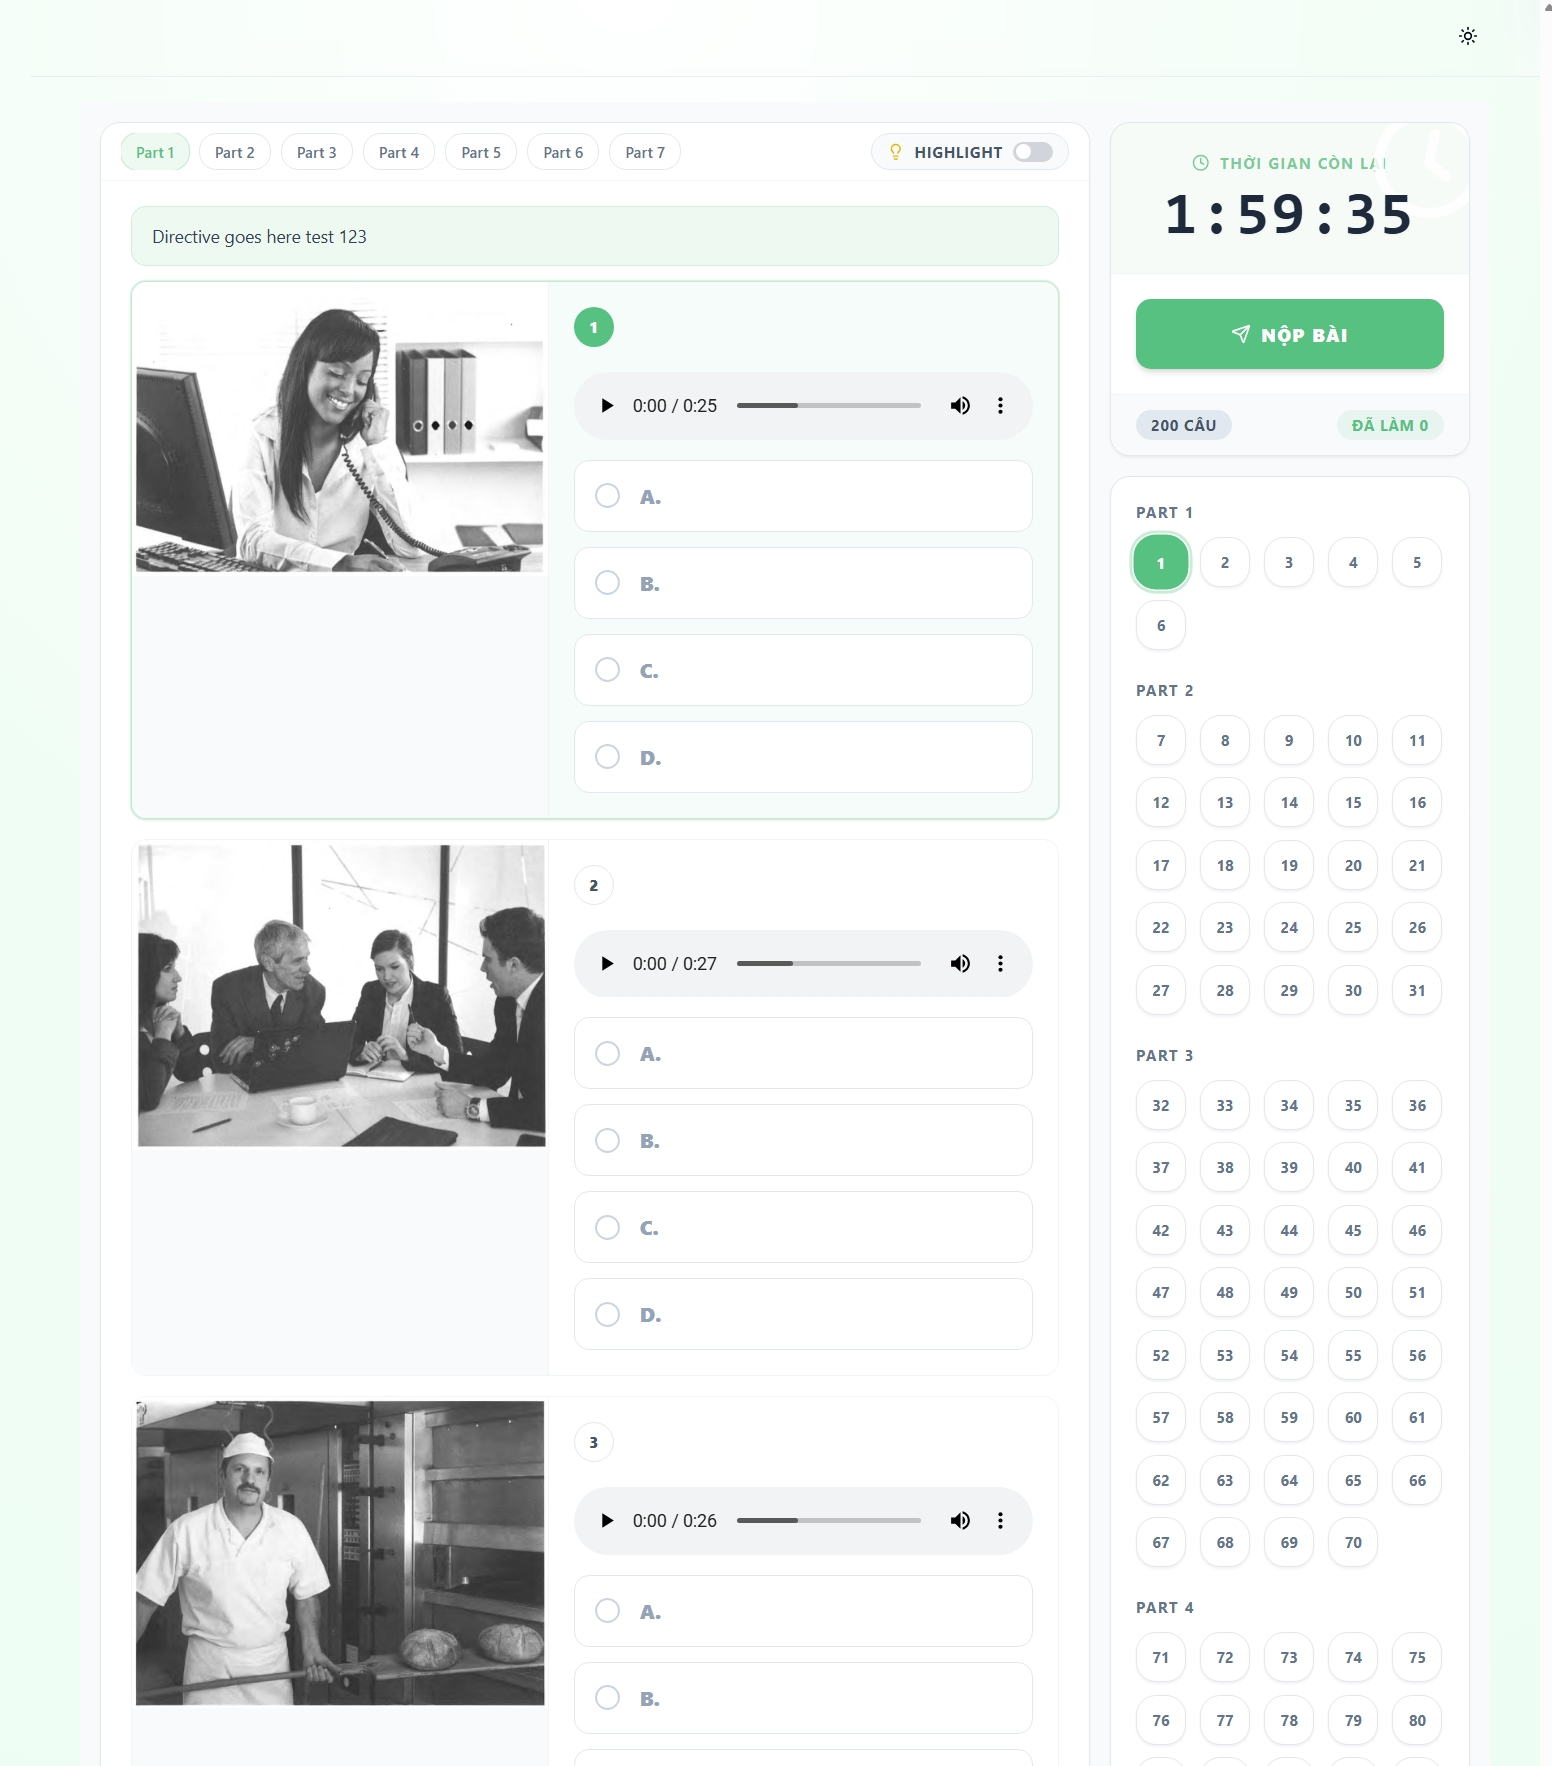
\includegraphics[width=0.75\linewidth]{graphics/ui/exam/exam-interface.jpg}
    \captionsetup{skip=5pt}
    \caption{Giao diện làm bài thi}
    \label{h12}
\end{figure}
\noindent Giao diện làm bài được thiết kế nhằm tạo ra môi trường tập trung và sát với trải nghiệm thi thật. Bố cục chia tách hợp lý giữa phần nội dung đọc và khu vực trả lời giúp người dùng vừa theo dõi đề bài vừa thao tác trả lời một cách thuận tiện. Các công cụ phụ trợ như bộ đếm thời gian và trình điều hướng câu hỏi hỗ trợ người học kiểm soát chiến lược làm bài hiệu quả hơn. Trong trường hợp muốn kết thúc sớm, người dùng có thể chủ động nộp bài thông qua nút "Nộp bài" được bố trí rõ ràng.

\begin{figure}[H]
    \centering
    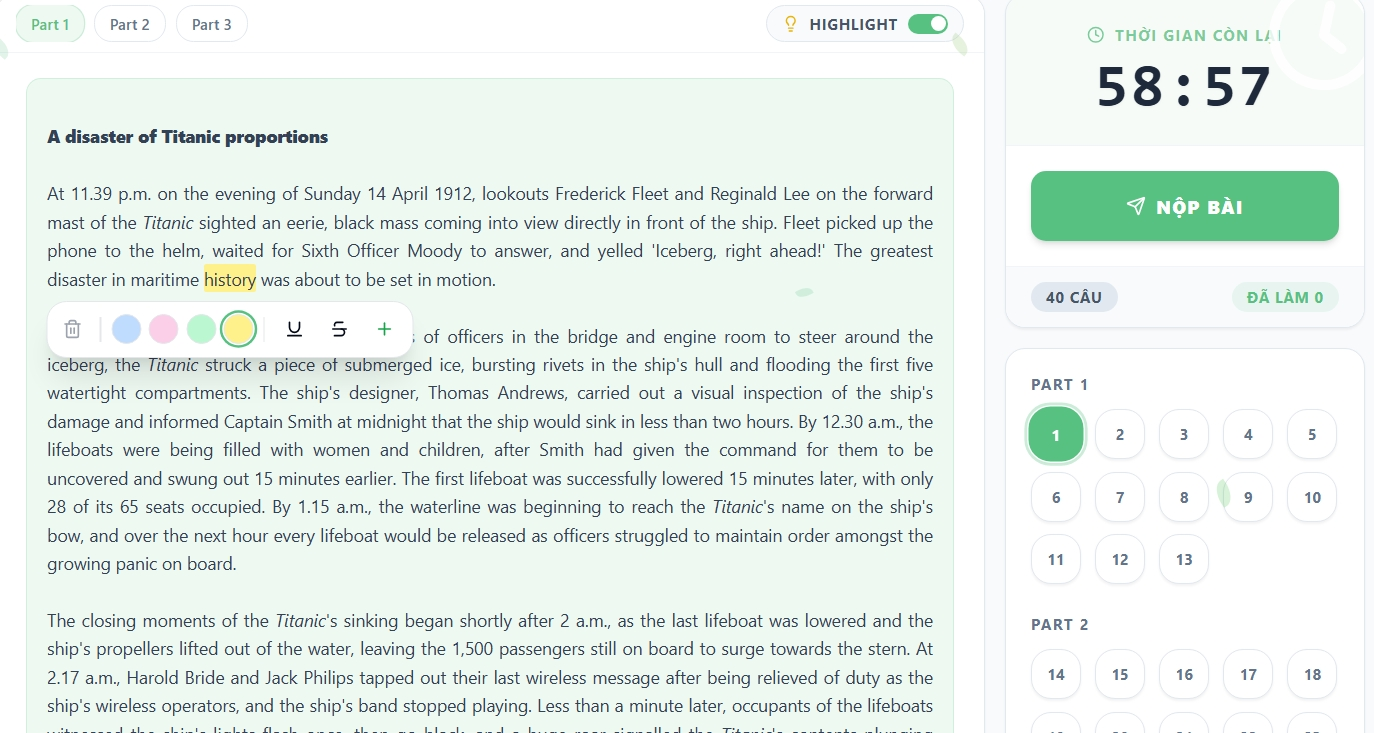
\includegraphics[width=0.75\linewidth]{graphics/ui/exam/exam-interface-highlight.jpg}
    \captionsetup{skip=5pt}
    \caption{Công cụ tô sáng và ghi chú văn bản}
    \label{h12_highlight}
\end{figure}
\noindent Bên cạnh chức năng làm bài cơ bản, hệ thống còn cung cấp bộ công cụ chú thích số nhằm nâng cao hiệu quả đọc hiểu trong quá trình luyện tập. Người dùng có thể tô sáng nhiều màu, định dạng văn bản hoặc tạo ghi chú trực tiếp từ đoạn văn đang đọc. Những công cụ này giúp học viên nhanh chóng đánh dấu ý chính, lưu lại bằng chứng quan trọng cho câu hỏi và tổ chức thông tin một cách có hệ thống hơn.

\begin{figure}[H]
    \centering
    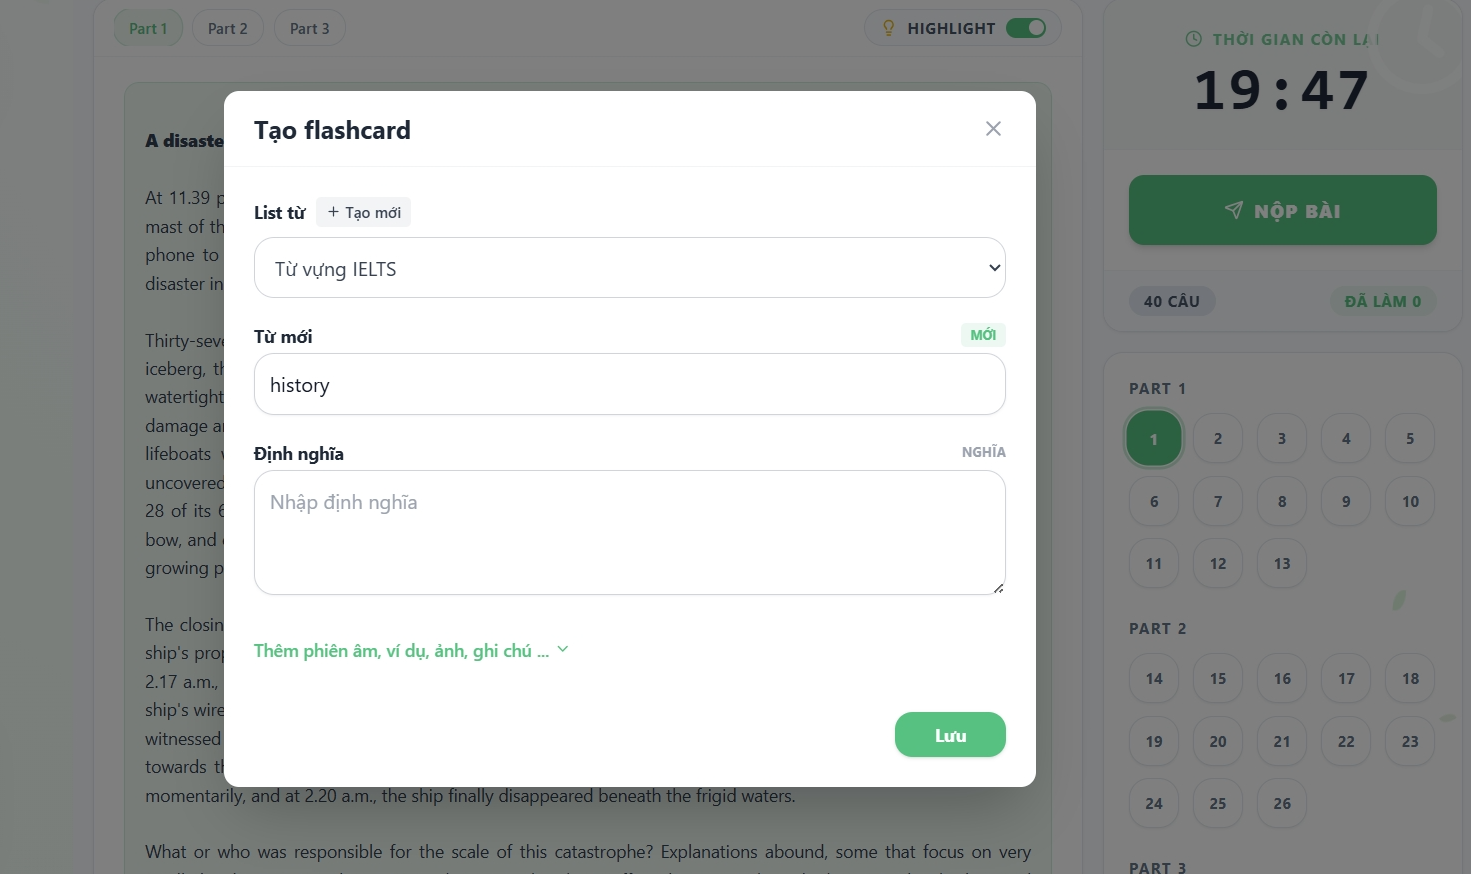
\includegraphics[width=0.75\linewidth]{graphics/ui/exam/exam-interface-create-flashcard.jpg}
    \captionsetup{skip=5pt}
    \caption{Tạo flashcard ngay trong lúc làm bài}
    \label{h12_flashcard}
\end{figure}
\noindent Một điểm nổi bật của hệ thống là khả năng tạo flashcard trực tiếp từ nội dung được tô sáng ngay trong bài thi. Tính năng này giúp giảm khoảng cách giữa quá trình phát hiện từ vựng mới và việc lưu trữ để ôn tập về sau. Hộp thoại tạo flashcard được thiết kế đơn giản, hỗ trợ lưu nhanh hoặc bổ sung ghi chú ngôn ngữ chi tiết, từ đó biến mỗi lần luyện đề thành một cơ hội tích lũy kiến thức lâu dài và có tính cá nhân hóa cao.

\begin{figure}[H]
    \centering
    
\includegraphics[width=0.75\linewidth]{graphics/ui/exam/exam-result.jpg}
    \captionsetup{skip=5pt}
    \caption{Kết quả và phân tích bài thi}
    \label{h13}
\end{figure}
\noindent Sau khi nộp bài, người dùng được đưa đến trang kết quả để xem lại toàn bộ phần làm của mình. Phần đầu trang hiển thị điểm TOEIC, thời gian làm bài, số câu đúng, số câu sai và số câu bỏ qua. Bên dưới là bảng phân tích chi tiết theo từng dạng câu hỏi, giúp người học nhìn ra mình đang yếu ở phần nào để ôn tập lại hiệu quả hơn.




\subsubsection{Thẻ ghi nhớ}

\begin{figure}[H]
    \centering
    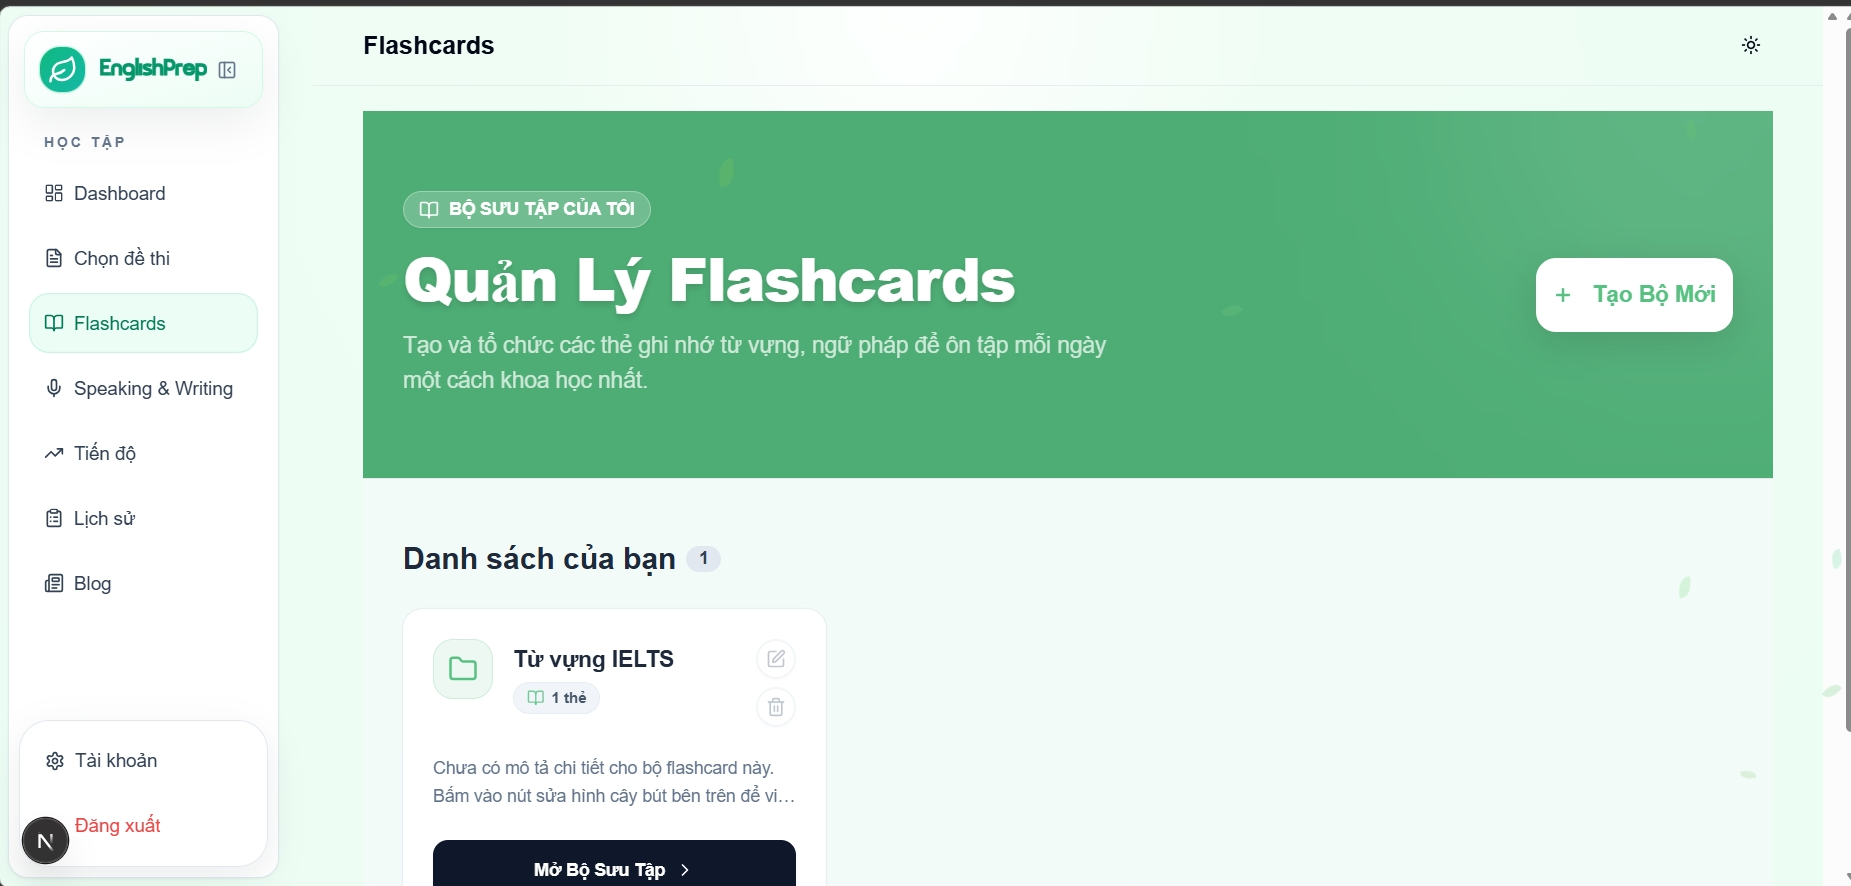
\includegraphics[width=0.75\linewidth]{graphics/ui/flashcard/flashcard-my-list.jpg}
    \captionsetup{skip=5pt}
    \caption{Danh sách bộ flashcard cá nhân}
    \label{h14}
\end{figure}
\noindent Đây là giao diện đầu mối cho hoạt động học từ vựng và ngữ pháp theo phương pháp flashcard trên nền tảng. Thiết kế sử dụng bố cục thanh bên kết hợp không gian làm việc chính để giúp người dùng phân loại nội dung theo từng nhóm học tập hoặc từng kỳ thi cụ thể. Nhờ đó, việc quản lý tài liệu ôn luyện trở nên có tổ chức và dễ mở rộng theo tiến độ học của từng cá nhân.


\begin{figure}[H]
    \centering
    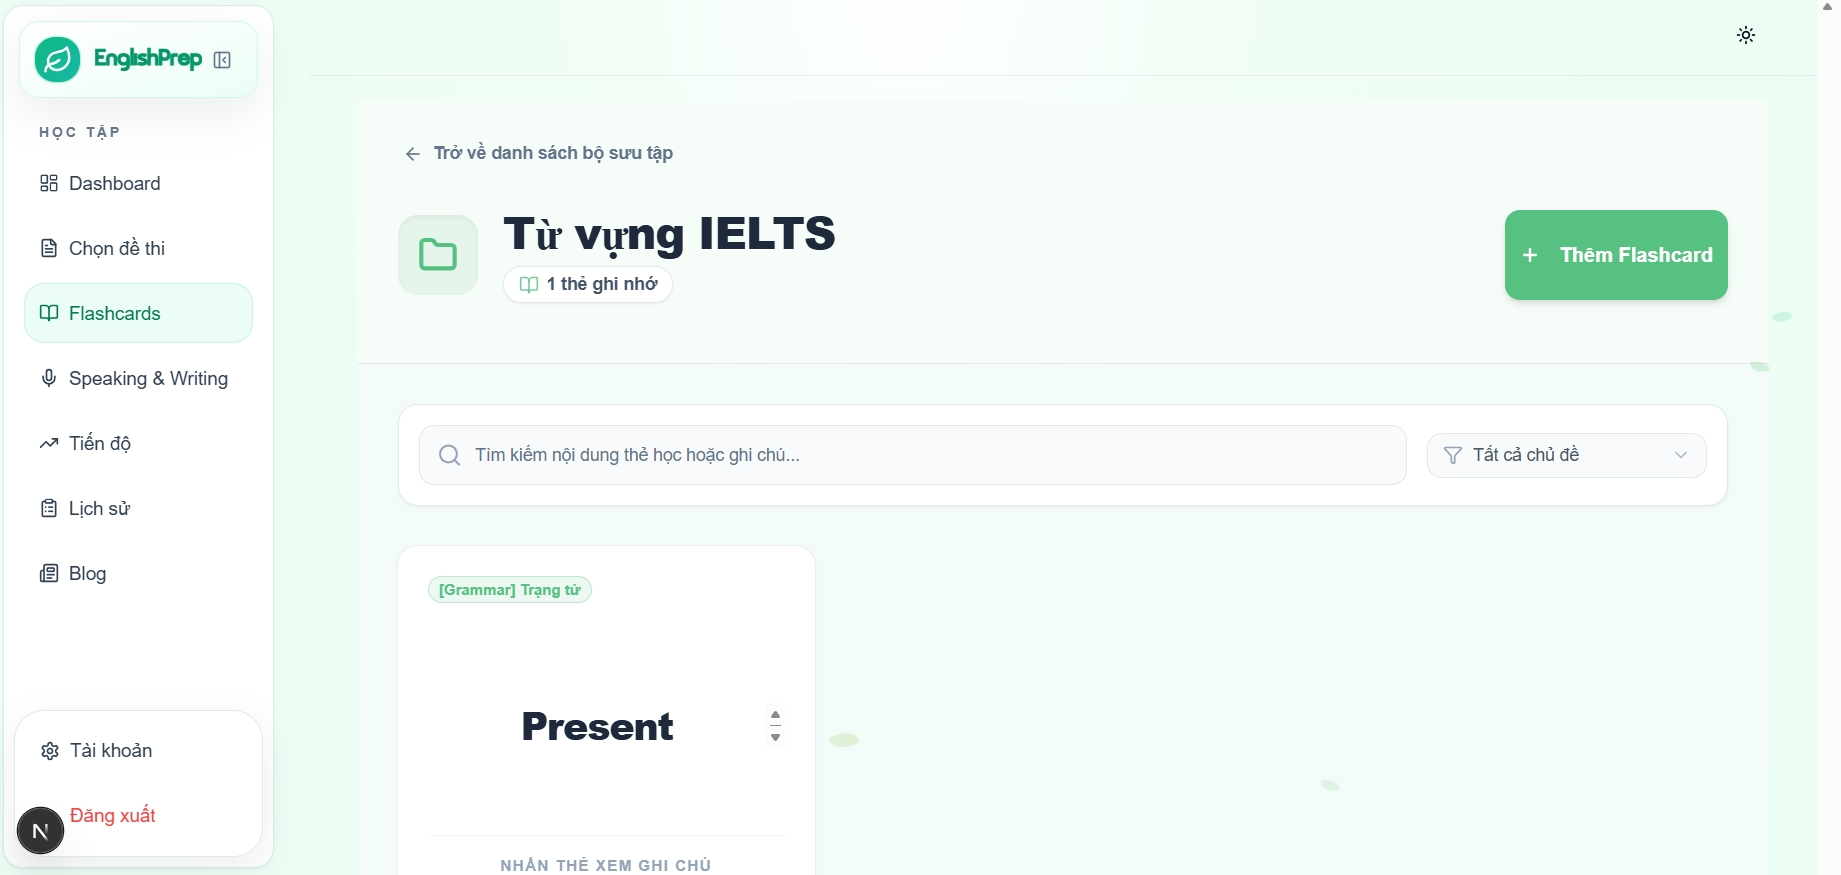
\includegraphics[width=0.75\linewidth]{graphics/ui/flashcard/flashcard-my-flashcard.jpg}
    \captionsetup{skip=5pt}
    \caption{Giao diện học với flashcard}
    \label{h15}
\end{figure}
\noindent Bảng điều khiển flashcard là trung tâm quản lý thư viện ngôn ngữ cá nhân của người học. Bố cục hai cột cân bằng giữa việc hiển thị phân loại tổng quát và quản lý chi tiết từng thẻ, đồng thời được hỗ trợ bởi chức năng tìm kiếm và lọc nội dung. Thiết kế này phù hợp với nhu cầu mở rộng vốn từ vựng theo thời gian mà vẫn giữ cho quá trình tra cứu và ôn tập diễn ra thuận tiện.

\begin{figure}[H]
    \centering
    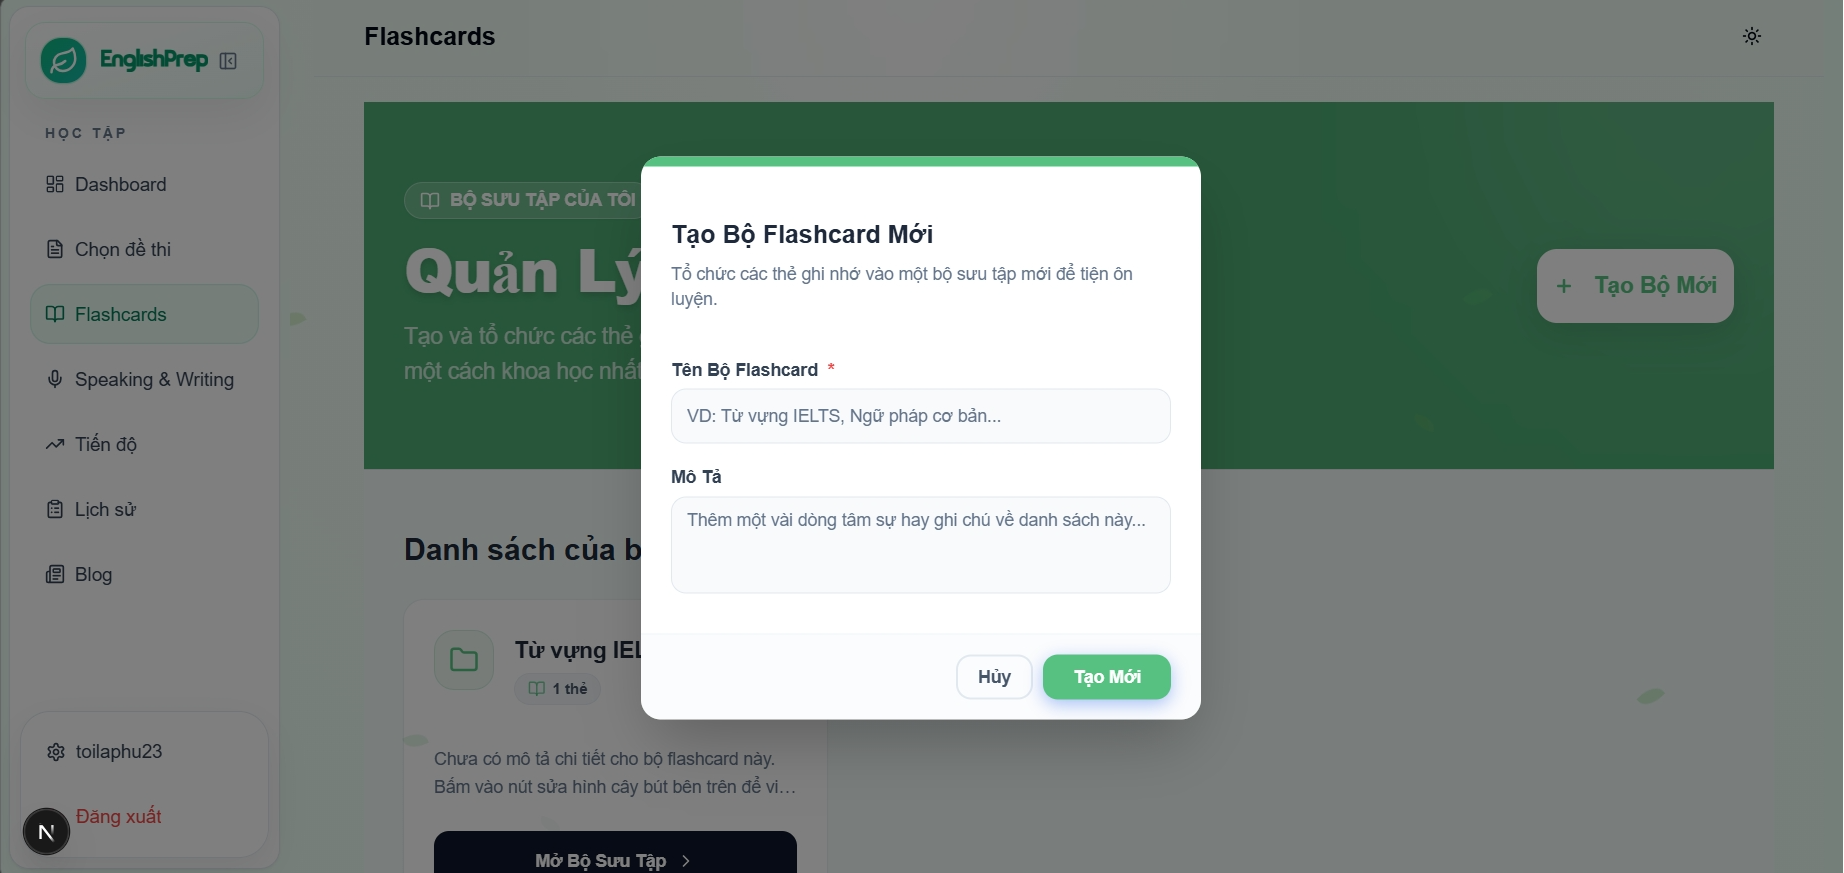
\includegraphics[width=0.75\linewidth]{graphics/ui/flashcard/flashcard-create-list.jpg}
    \captionsetup{skip=5pt}
    \caption{Tạo danh sách flashcard mới}
    \label{h17}
\end{figure}
\noindent Giao diện tạo danh sách mới hỗ trợ người dùng nhóm các tài liệu học thành những bộ có chủ đề riêng biệt. Việc cho phép đặt tên và thêm mô tả chi tiết giúp học viên tổ chức nội dung theo mục tiêu học tập, dạng đề hoặc nhóm từ vựng cụ thể. Điều này góp phần duy trì tính hệ thống và khả năng truy cập nhanh đối với tài liệu ôn luyện.

\begin{figure}[H]
    \centering
    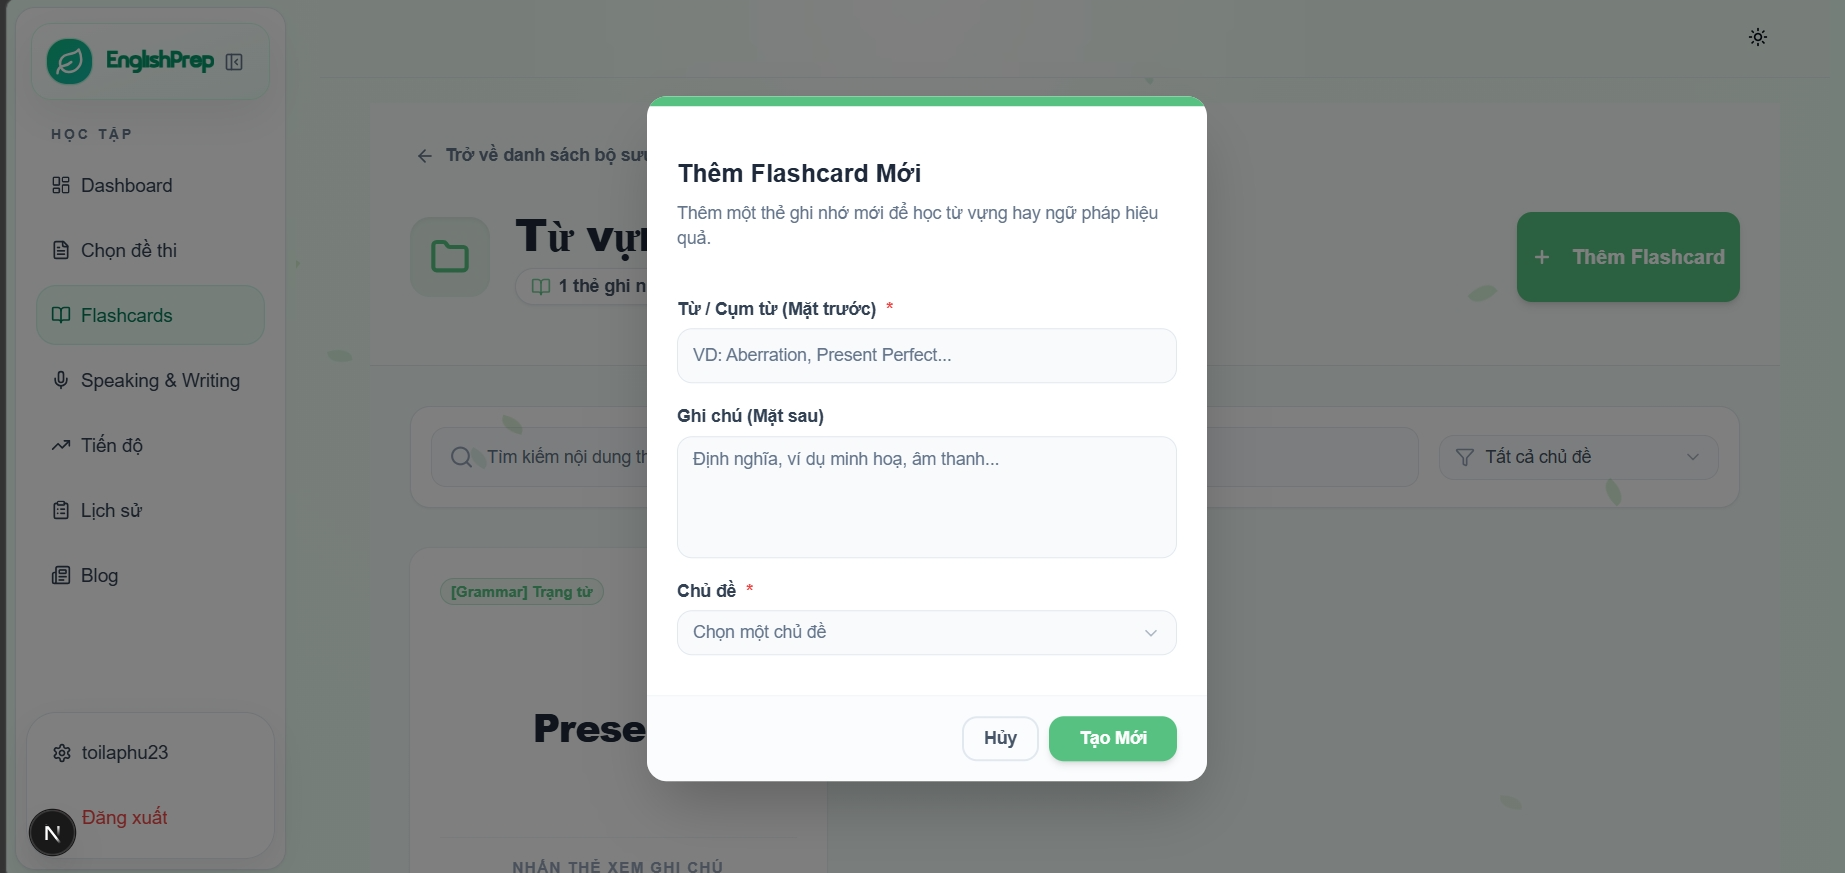
\includegraphics[width=0.75\linewidth]{graphics/ui/flashcard/flashcard-create-flashcard.jpg}
    \captionsetup{skip=5pt}
    \caption{Thêm flashcard mới}
    \label{h18}
\end{figure}
\noindent Hộp thoại thêm flashcard mới là công cụ đơn giản nhưng hiệu quả cho việc tự xây dựng nội dung học tập. Người dùng cần chọn danh sách, chủ đề và nhập thuật ngữ hoặc nội dung ghi nhớ, từ đó bảo đảm rằng hệ thống flashcard luôn được tổ chức nhất quán. Trường ghi chú tùy chọn còn cho phép bổ sung mẹo học, ví dụ hoặc liên tưởng cá nhân để tăng hiệu quả ghi nhớ.

\subsubsection{Luyện nói}

\begin{figure}[H]
    \centering
    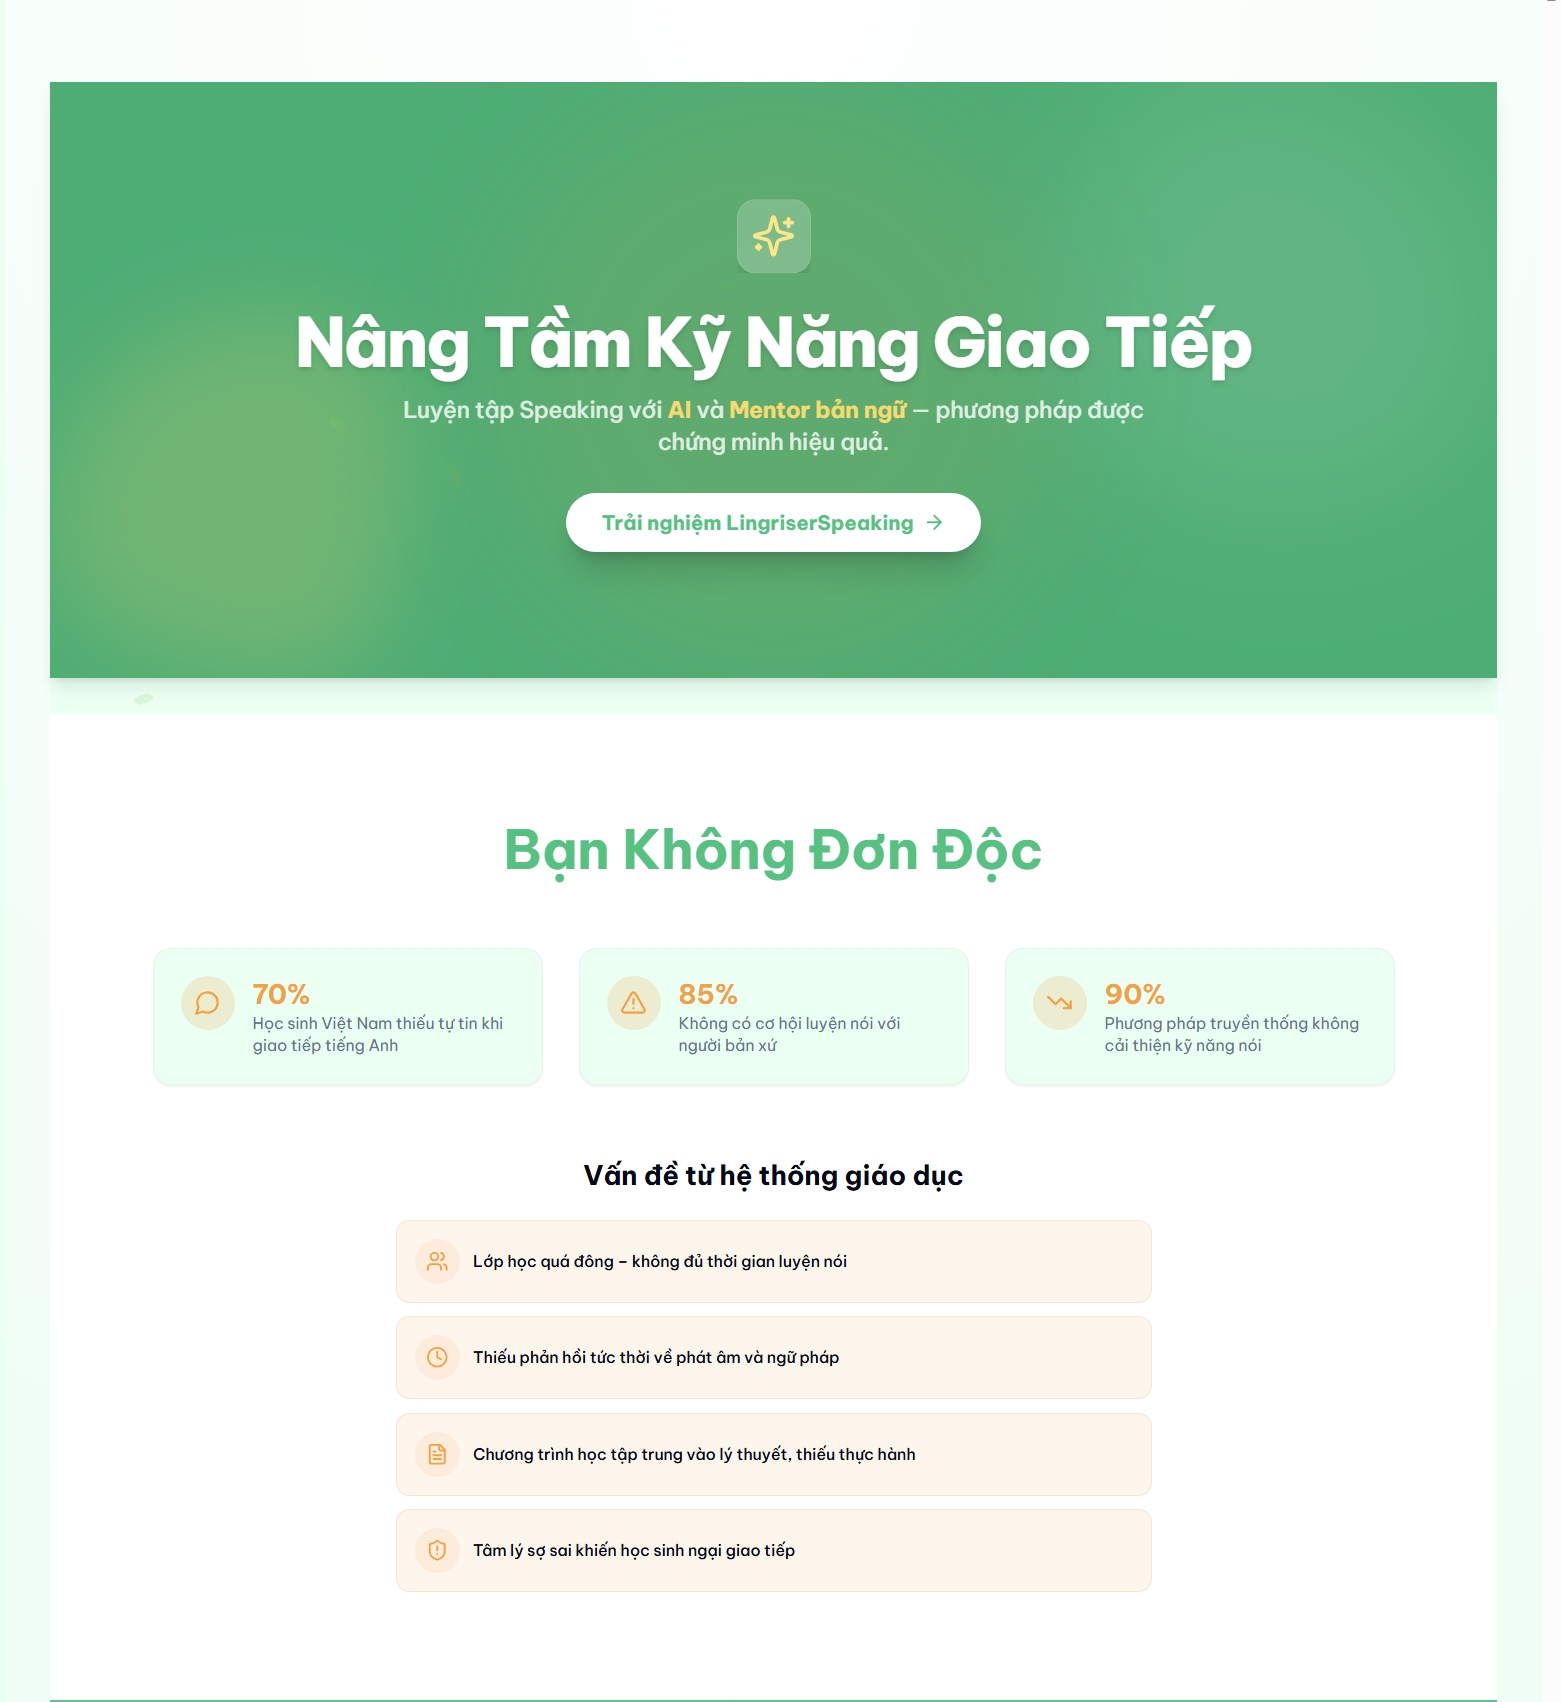
\includegraphics[width=0.75\linewidth]{graphics/ui/LingriserSpeaking/speaking-landing.jpg}
    \captionsetup{skip=5pt}
    \caption{Trang giới thiệu LingriserSpeaking}
    \label{fig:lingriser-speaking-landing}
\end{figure}
\noindent Trang này đóng vai trò như màn hình giới thiệu cho LingriserSpeaking. Phần đầu trang làm nổi bật thông điệp nâng cao kỹ năng giao tiếp cùng nút trải nghiệm để người dùng bắt đầu nhanh. Bên dưới là các số liệu và nhóm nội dung mô tả những khó khăn phổ biến khi học nói, qua đó làm rõ giá trị mà nền tảng muốn giải quyết. Cách trình bày này giúp người xem hiểu nhanh mục tiêu của sản phẩm và tạo động lực để tiếp tục khám phá các tính năng luyện nói.

\subsubsection{Tiến độ học tập}
\begin{figure}[H]
    \centering
    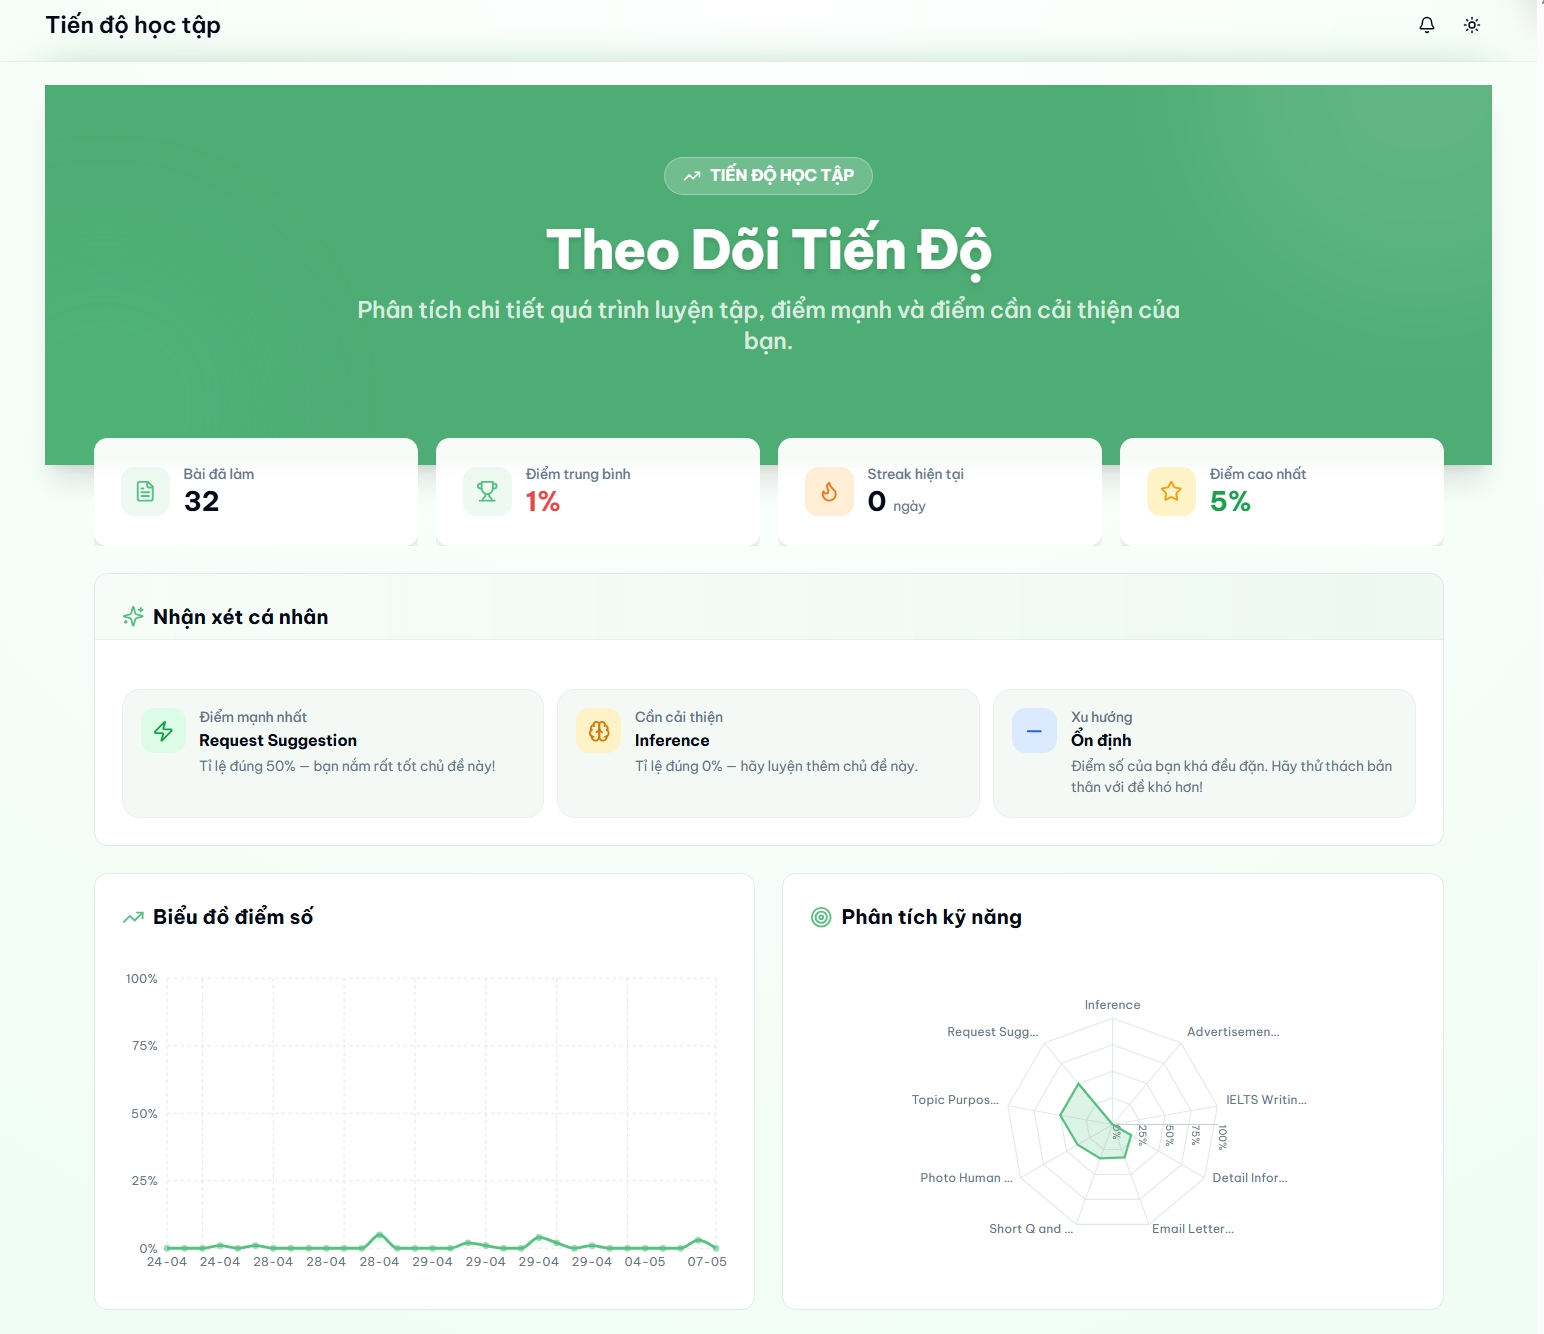
\includegraphics[width=0.75\linewidth]{graphics/ui/profile/profile-progress.jpg}
    \captionsetup{skip=5pt}
    \caption{Tiến độ học tập}
    \label{fig:profile-progress}
\end{figure}
\noindent Trang tiến độ học tập giúp người dùng nhìn nhanh quá trình ôn luyện của mình. Phần đầu trang hiển thị các chỉ số quan trọng như số đề đã làm, điểm trung bình, chuỗi học tập và điểm cao nhất. Bên dưới là các biểu đồ, nhận xét cá nhân và bảng phân tích theo từng kỹ năng hoặc chủ đề, giúp người học dễ nhận ra điểm mạnh, điểm yếu và theo dõi sự cải thiện theo thời gian.

\subsubsection{Hồ sơ cá nhân}

\begin{figure}[H]
    \centering
    
\includegraphics[width=0.75\linewidth]{graphics/ui/profile/profile-overview.jpg}
    \captionsetup{skip=5pt}
    \caption{Tổng quan hồ sơ cá nhân}
\end{figure}
\noindent Giao diện tổng quan hồ sơ cá nhân được thiết kế như trung tâm theo dõi tiến độ và quản lý thông tin học tập của người dùng. Phần đầu trang hiển thị ảnh đại diện, tên tài khoản, email, ngày tham gia cùng các nút thao tác nhanh như cập nhật hồ sơ, phân tích học tập và đổi mật khẩu. Ngay bên dưới là khu vực mục tiêu cá nhân, giúp người học theo dõi hoặc bổ sung các mục tiêu mới trong quá trình ôn luyện. Phần nội dung chính được chia theo các thẻ chức năng; tại thẻ ``Thống kê \& Tổng quan'', hệ thống trình bày biểu đồ phân tích theo chủ đề, thẻ chuỗi học tập và các chỉ số hiệu suất theo từng nhóm kỹ năng, từ đó giúp người dùng nhìn rõ mức độ tiến bộ của mình một cách trực quan và liên tục.

\begin{figure}[H]
    \centering
    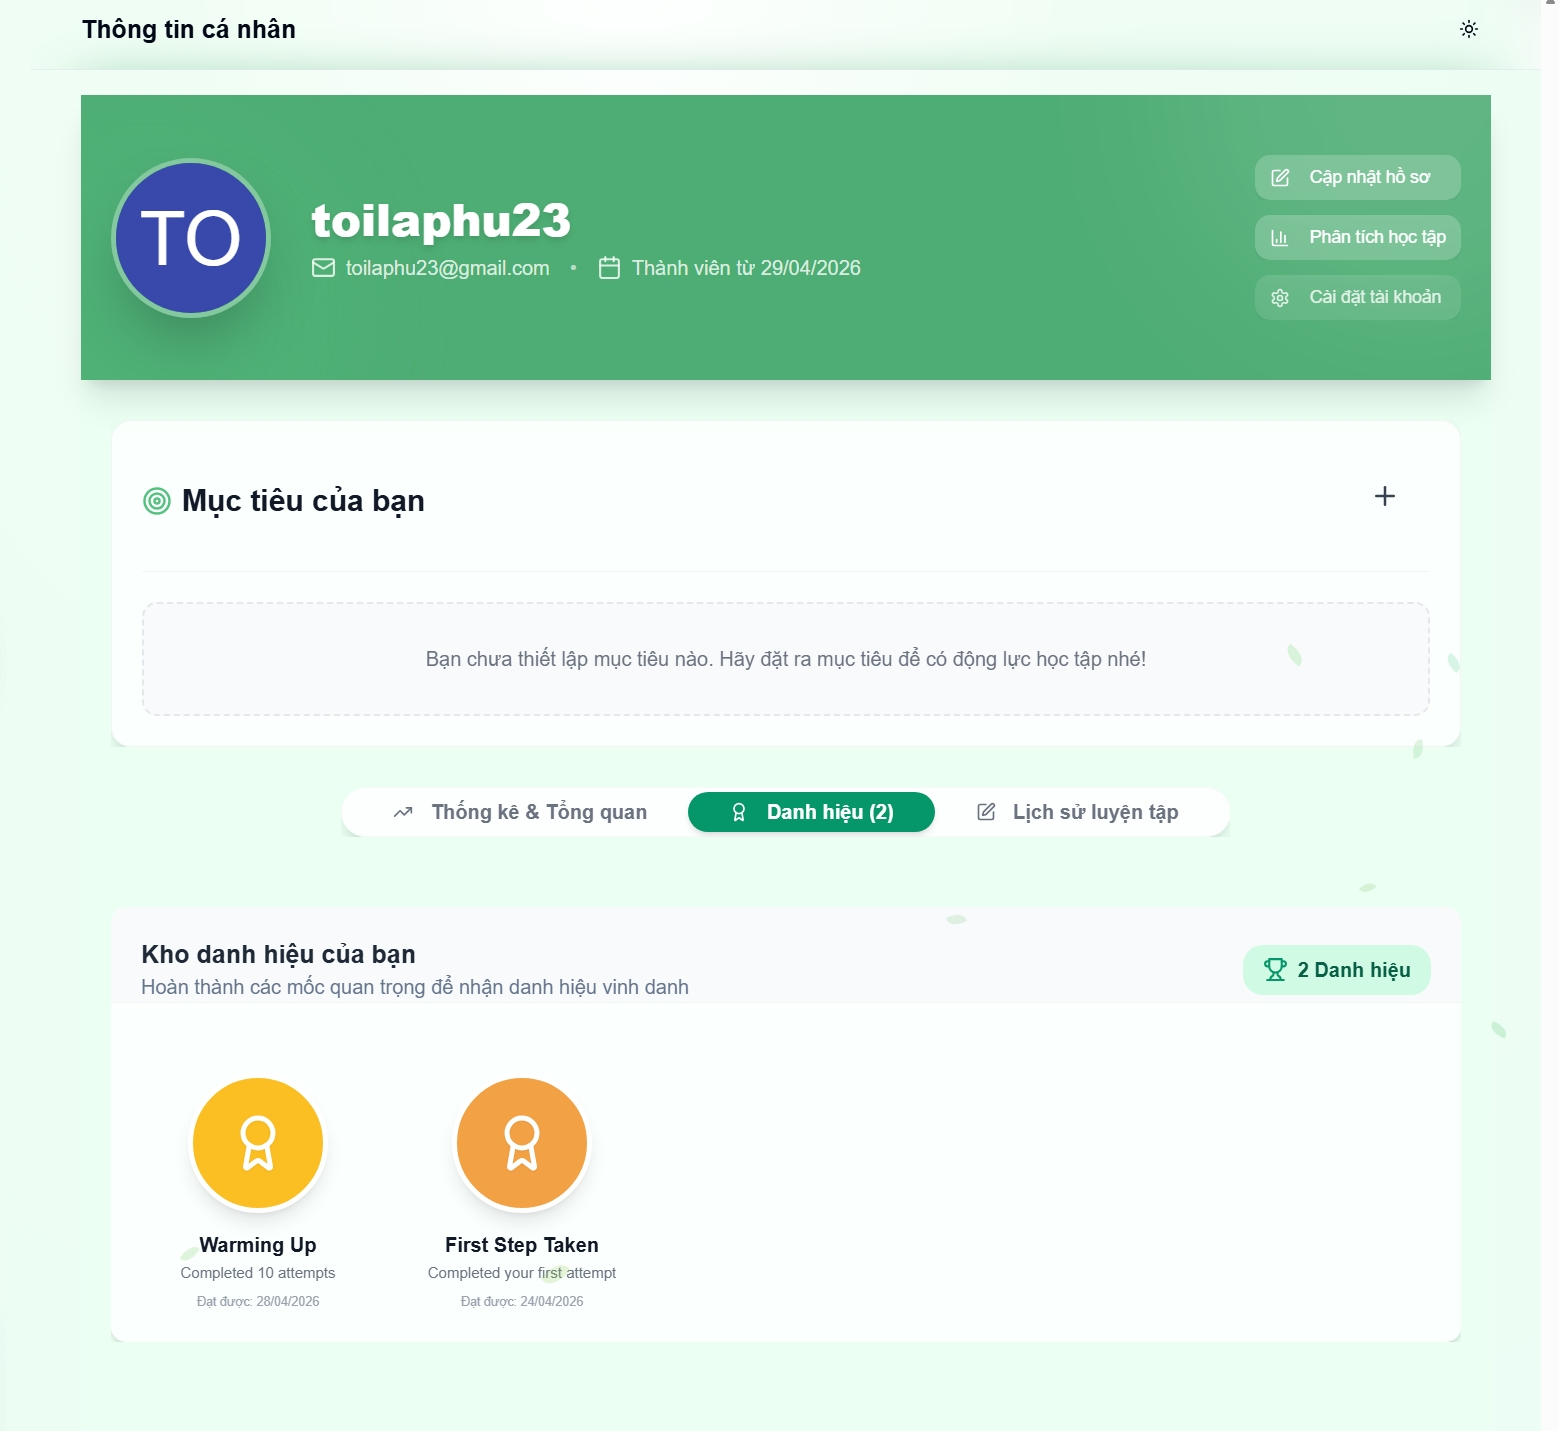
\includegraphics[width=0.75\linewidth]{graphics/ui/profile/profile-achievement.jpg}
    \captionsetup{skip=5pt}
    \caption{Danh hiệu trong hồ sơ cá nhân}
    \label{fig:profile-achievement}
\end{figure}
\noindent Ở thẻ ``Danh hiệu'', hồ sơ cá nhân chuyển trọng tâm từ thống kê sang động lực học tập. Giao diện liệt kê các huy hiệu mà người dùng đã mở khóa, kèm theo tên danh hiệu, điều kiện đạt được và thời điểm nhận thưởng. Cách tổ chức này giúp biến tiến trình luyện tập thành các cột mốc dễ ghi nhớ, đồng thời khuyến khích người học duy trì tần suất làm bài để chinh phục thêm các thành tích mới.



\begin{figure}[H]
    \centering
    
\includegraphics[width=0.75\linewidth]{graphics/ui/profile/profile-history.jpg}
    \captionsetup{skip=5pt}
    \caption{Lịch sử học tập}
    \label{h21}
\end{figure}
\noindent Trang lịch sử làm bài được thiết kế để người dùng xem lại toàn bộ các bài đã hoàn thành một cách rõ ràng và thuận tiện. Phần đầu trang nổi bật với tiêu đề lớn và các thẻ thống kê nhanh như tổng số bài, số bài hoàn thành, điểm trung bình và điểm cao nhất. Ngay bên dưới là khu vực sắp xếp, giúp người học lọc hoặc xem lại kết quả theo thứ tự phù hợp. Phần nội dung chính hiển thị danh sách chi tiết các bài đã làm, trong đó mỗi mục cho biết tên bài, thời gian hoàn thành, điểm số, số câu đúng hoặc thời lượng làm bài, kèm nút ``Xem chi tiết'' để mở lại kết quả. Cách bố trí này giúp người học dễ theo dõi tiến trình ôn luyện và nhanh chóng tìm lại những bài cần xem lại.

\begin{figure}[H]
    \centering
    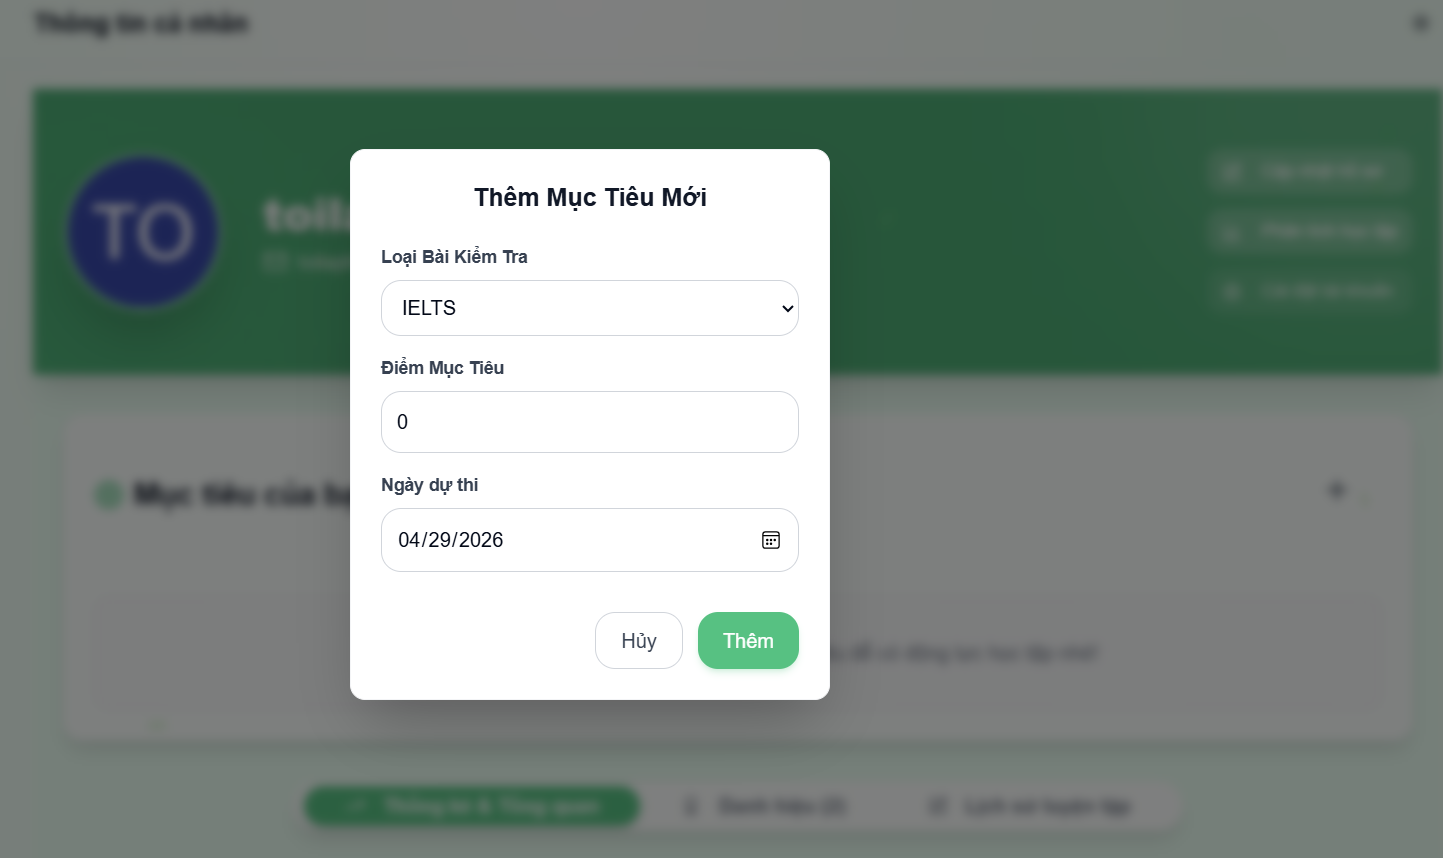
\includegraphics[width=0.75\linewidth]{graphics/ui/profile/profile-add-goal.jpg}
    \captionsetup{skip=5pt}
    \caption{Hộp thoại thiết lập mục tiêu}
    \label{fig:profile-add-goal}
\end{figure}
\noindent Hộp thoại thiết lập mục tiêu cho phép người dùng bổ sung nhanh các cột mốc học tập ngay trong trang hồ sơ mà không cần rời khỏi luồng theo dõi tiến độ. Biểu mẫu tập trung vào các thông tin thiết yếu như tên mục tiêu, loại kỳ thi, điểm mong muốn và thời hạn hoàn thành, giúp việc đặt mục tiêu trở nên rõ ràng và có thể đo lường được. Việc tích hợp thao tác này trực tiếp trong hồ sơ cá nhân giúp người học dễ dàng liên kết kế hoạch dài hạn với dữ liệu luyện tập thực tế đang được hệ thống ghi nhận.

\subsubsection{Bài viết}

\begin{figure}[H]
    \centering
    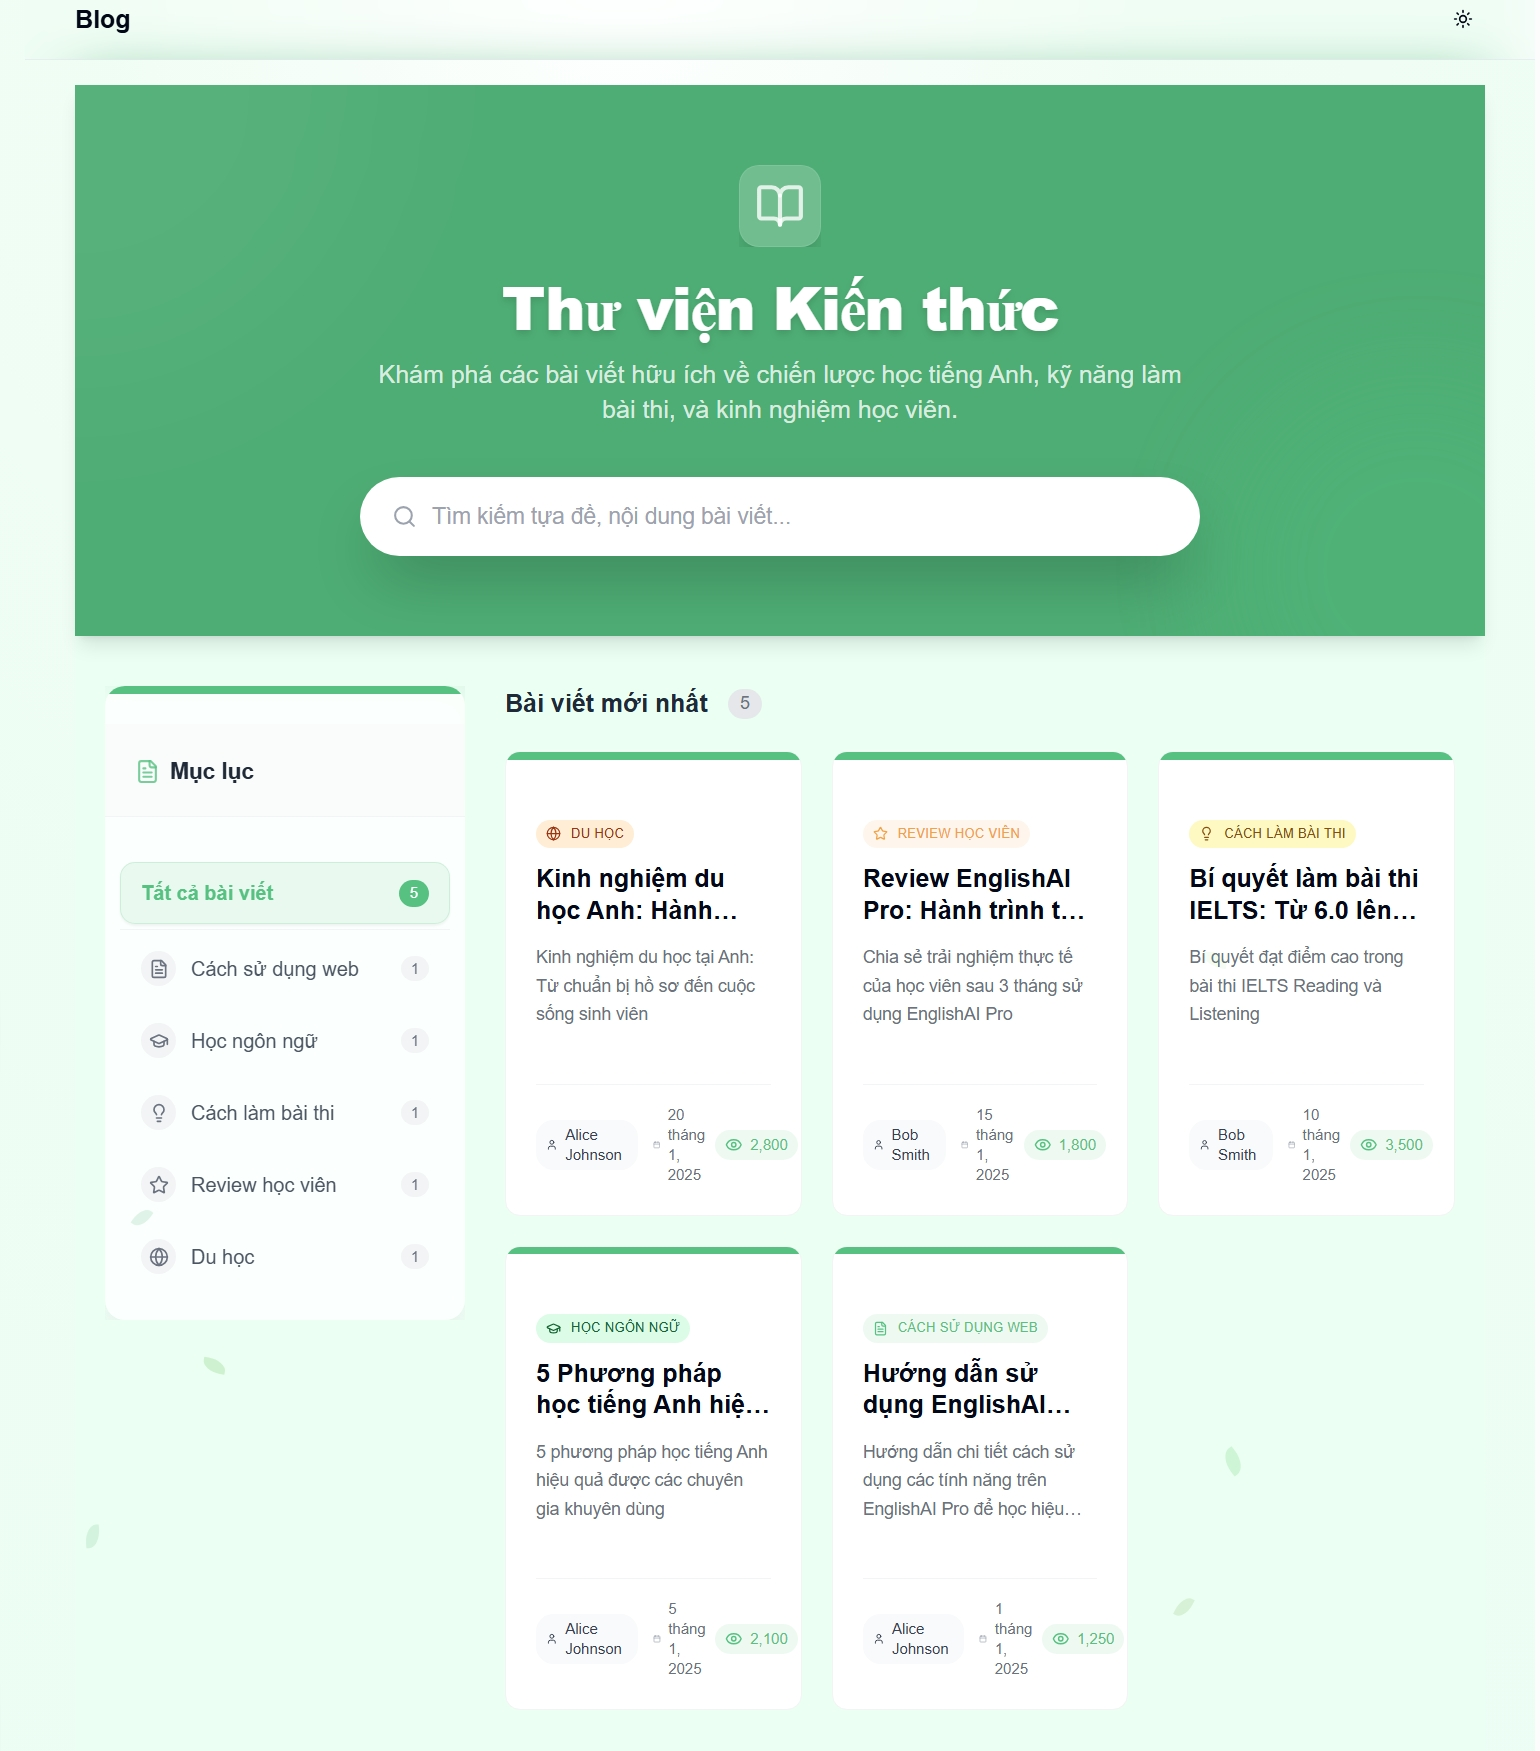
\includegraphics[width=0.75\linewidth]{graphics/ui/blog/blog-selection.jpg}
    \captionsetup{skip=5pt}
    \caption{Danh sách bài viết blog}
    \label{fig:blog-selection}
\end{figure}
\noindent Giao diện blog hoạt động như một trung tâm khám phá nội dung học tập trong hệ thống. Các bài viết được sắp xếp theo dạng lưới dễ quan sát, đi kèm thanh bên hỗ trợ lọc theo chủ đề và các thẻ nội dung tóm tắt thông tin quan trọng của từng bài. Cách tổ chức này giúp người dùng nhanh chóng chuyển đổi giữa các nhóm chủ đề như mẹo luyện thi IELTS, hướng dẫn sử dụng nền tảng hoặc các bài chia sẻ kiến thức liên quan.

\begin{figure}[H]
    \centering
    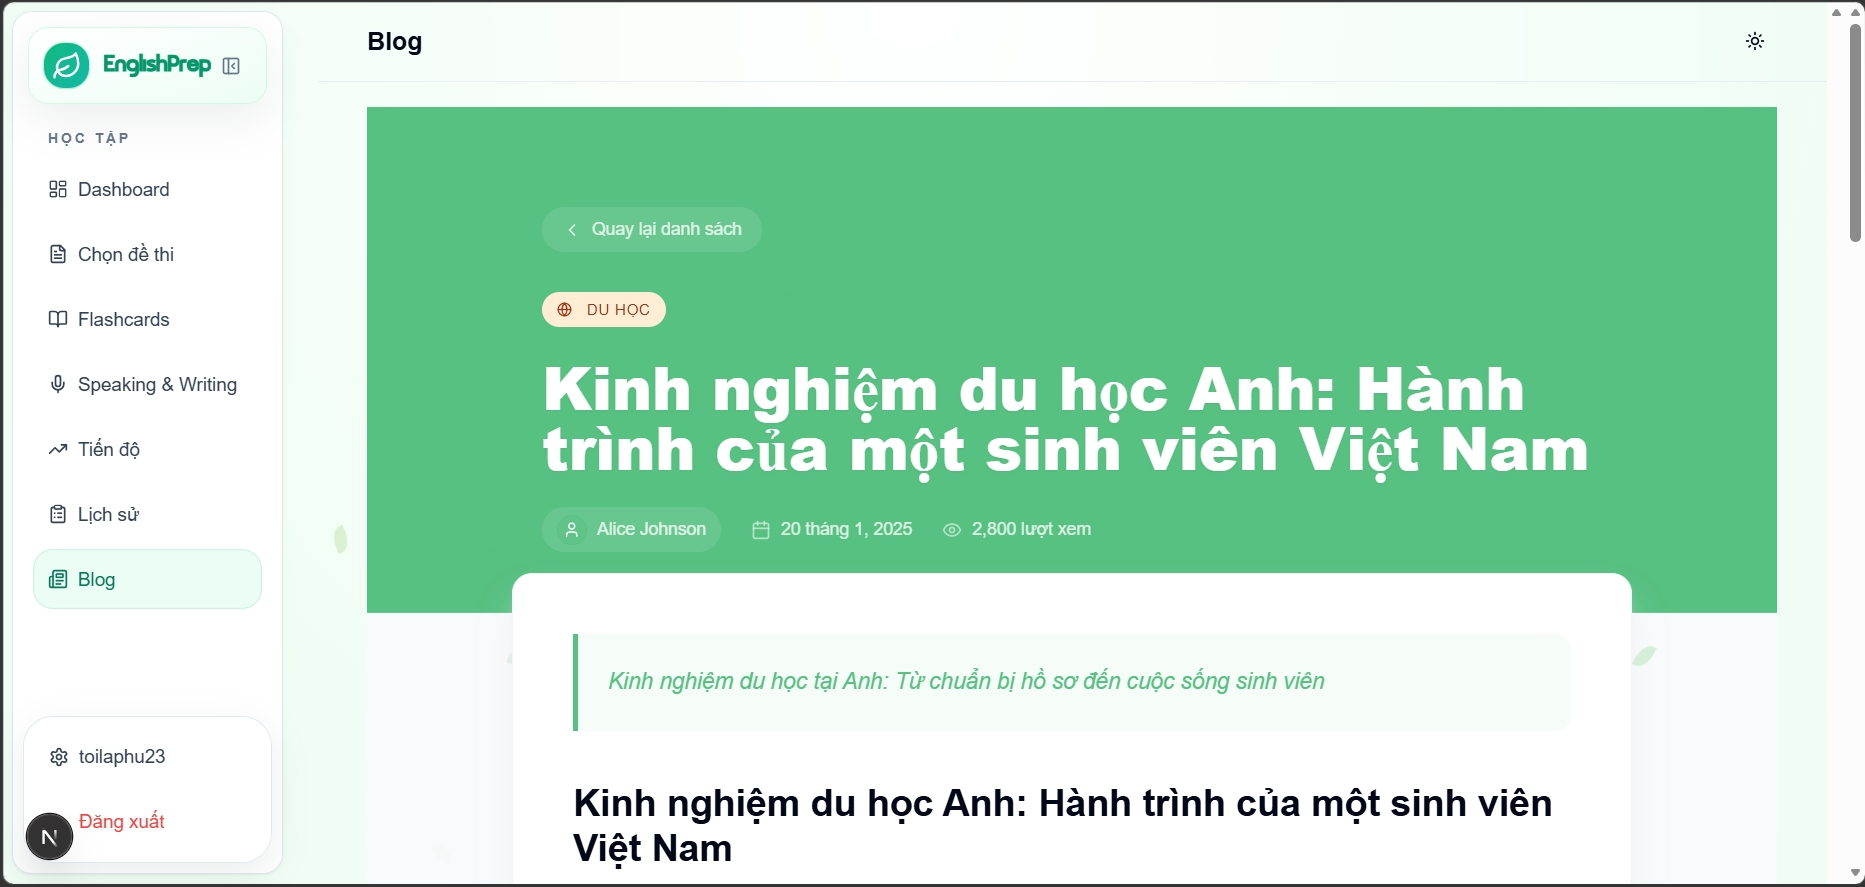
\includegraphics[width=0.75\linewidth]{graphics/ui/blog/blog-example.jpg}
    \captionsetup{skip=5pt}
    \caption{Trang chi tiết bài viết blog}
    \label{fig:blog-example}
\end{figure}
\noindent Trang hiển thị bài viết blog được thiết kế theo hướng dễ đọc và chuyên nghiệp. Quản trị viên hoặc người tạo nội dung có thể trình bày bài viết bằng cấu trúc phân cấp gồm tiêu đề, đề mục và danh sách gạch đầu dòng để truyền tải thông tin dài một cách rõ ràng. Sự kết hợp giữa điều hướng tiêu chuẩn, thông tin bài viết và nội dung chính giúp tạo nên trải nghiệm đọc mạch lạc và hấp dẫn đối với người dùng.

\subsubsection{Trò chuyện}
\begin{figure}[H]
    \centering
    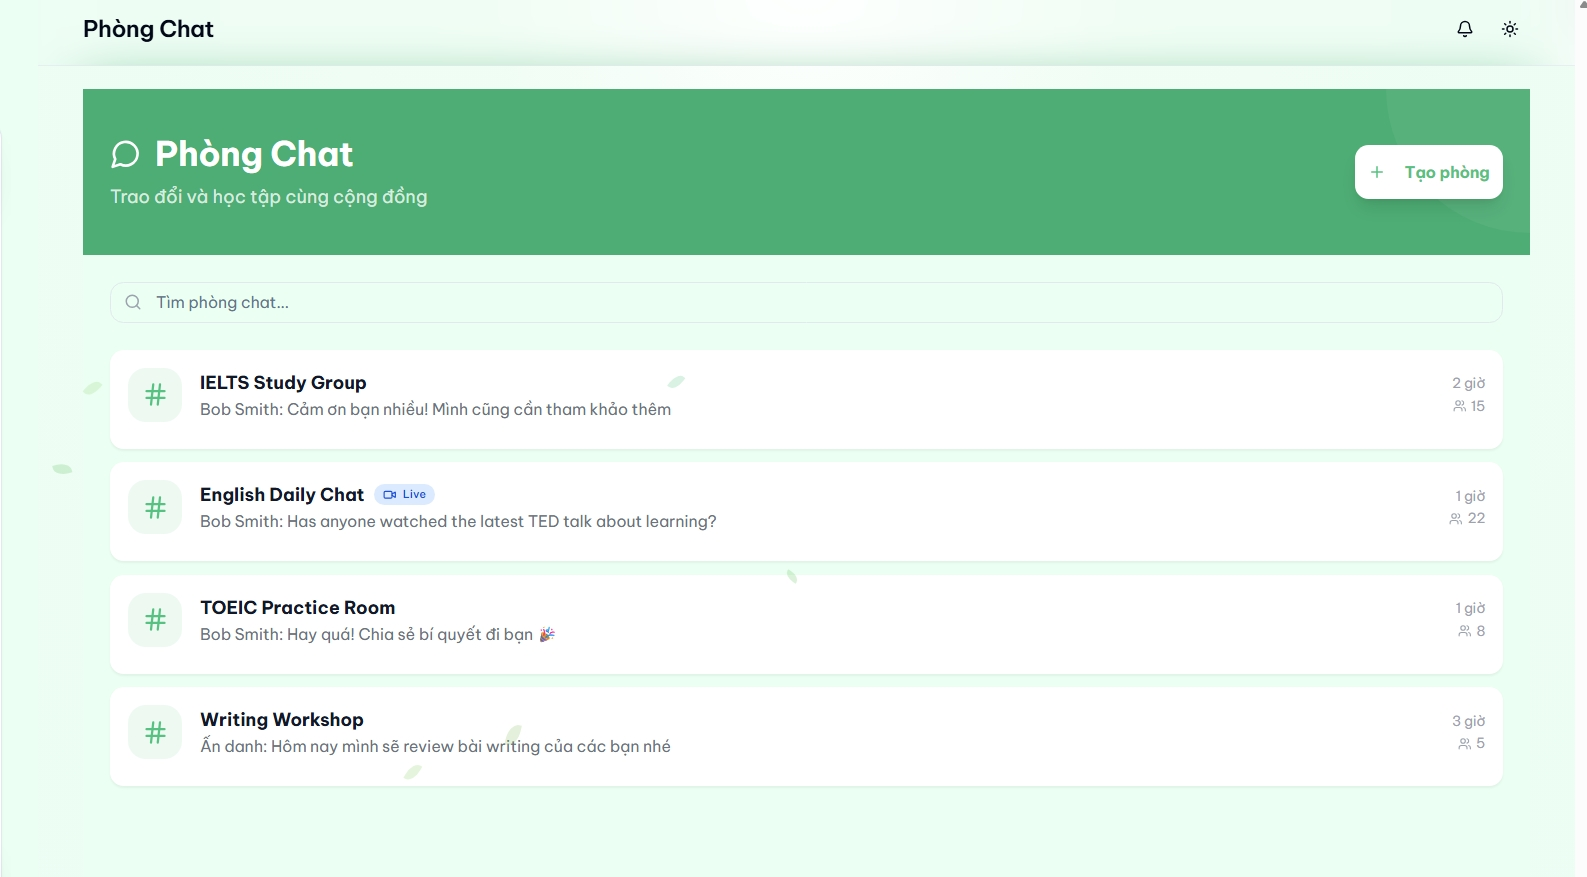
\includegraphics[width=0.75\linewidth]{graphics/ui/chat/chat.jpg}
    \captionsetup{skip=5pt}
    \caption{Danh sách phòng chat cộng đồng}
    \label{fig:chat-room-list}
\end{figure}
\noindent Giao diện phòng chat được thiết kế theo hướng thân thiện, gọn gàng và dễ theo dõi. Phần đầu trang làm nổi bật tiêu đề khu vực cùng nút ``Tạo phòng'', giúp người dùng nhanh chóng bắt đầu một không gian trao đổi mới. Ngay bên dưới là thanh tìm kiếm để lọc phòng chat theo nhu cầu. Danh sách các phòng được trình bày dưới dạng thẻ với tên phòng, đoạn tin nhắn gần nhất, thời gian cập nhật và số lượng thành viên đang tham gia; một số phòng còn có nhãn ``Live'' để nhấn mạnh mức độ hoạt động tức thời. Cách bố trí này giúp người học dễ tìm đúng cộng đồng thảo luận, theo dõi hoạt động mới và tham gia trao đổi một cách thuận tiện.

\subsection{Giao diện tính năng cho admin}

\subsubsection{Bảng điều khiển}

\begin{figure}[H]
    \centering
    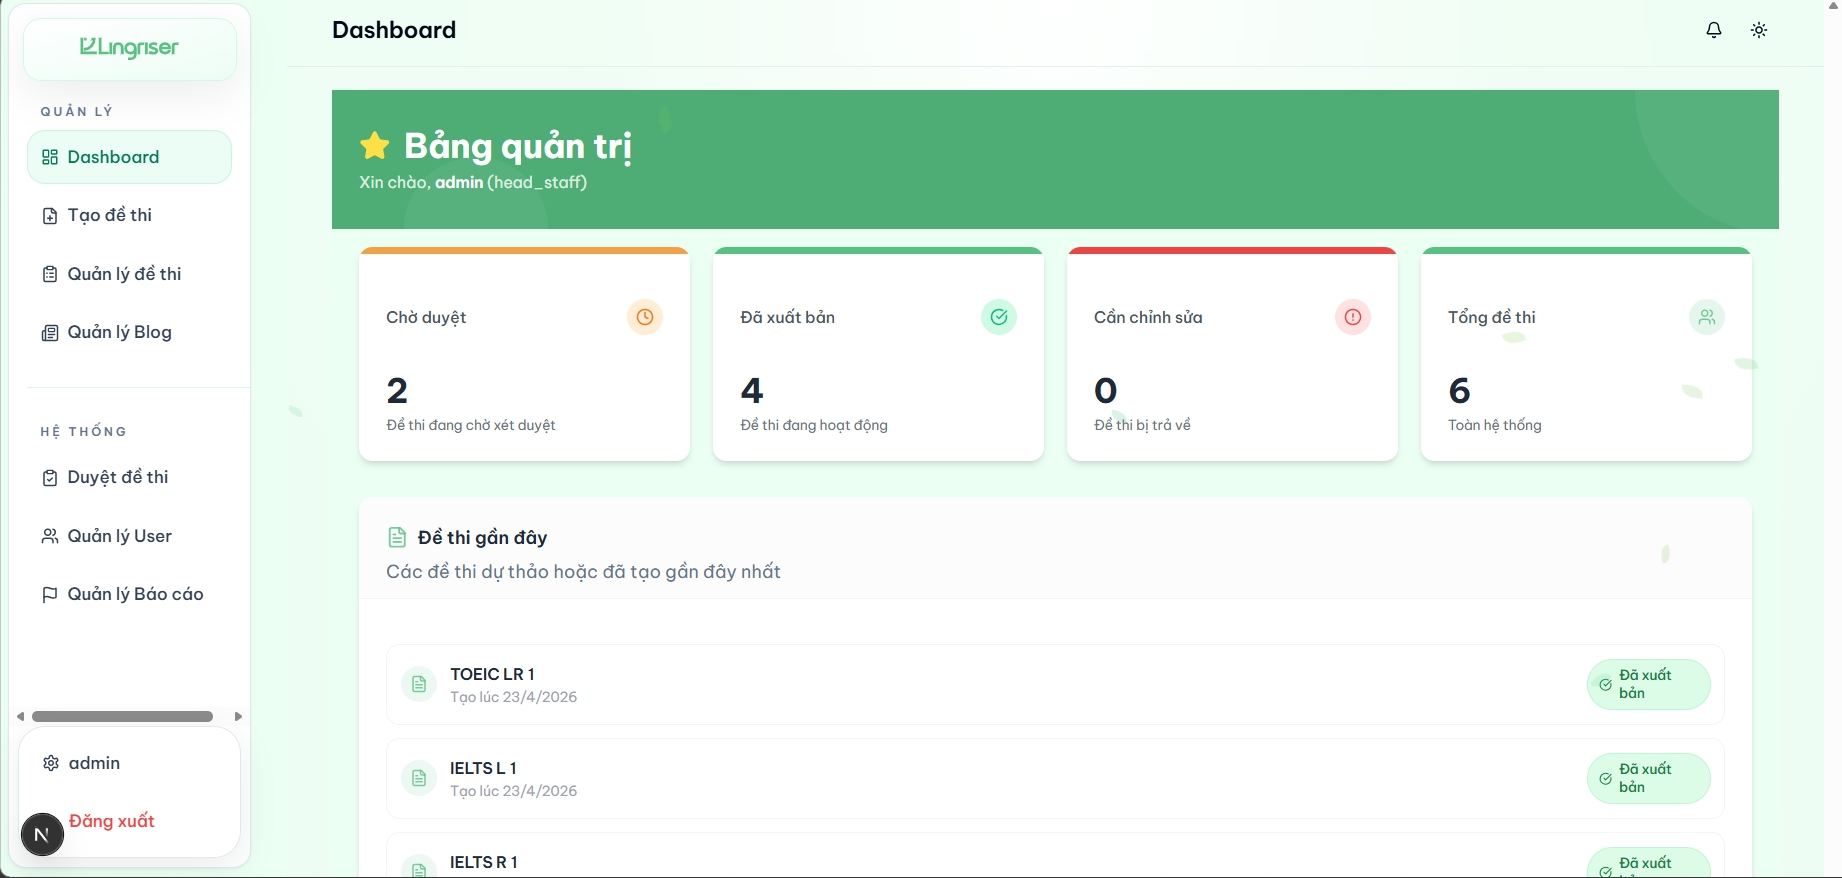
\includegraphics[width=0.75\linewidth]{graphics/ui/admin/admin-dashboard.jpg}
    \captionsetup{skip=5pt}
    \caption{Bảng điều khiển quản trị}
    \label{fig:admin-dashboard}
\end{figure}

\noindent Bảng điều khiển quản trị là nơi quản trị viên theo dõi nhanh tình trạng vận hành của hệ thống. Giao diện có thanh menu bên trái để truy cập các chức năng như tạo đề thi, quản lý đề thi, duyệt đề, quản lý người dùng và báo cáo. Ở phần nội dung chính, hệ thống hiển thị các thẻ thống kê như số đề chờ duyệt, số đề đã xuất bản, số đề cần chỉnh sửa và tổng số đề hiện có. Bên dưới là danh sách các đề thi gần đây, giúp quản trị viên dễ theo dõi và xử lý công việc hằng ngày.


\subsubsection{Tạo đề thi}

\begin{figure}[H]
    \centering
    \IfFileExists{graphics/ui/admin/exam-creation.jpg}{%
        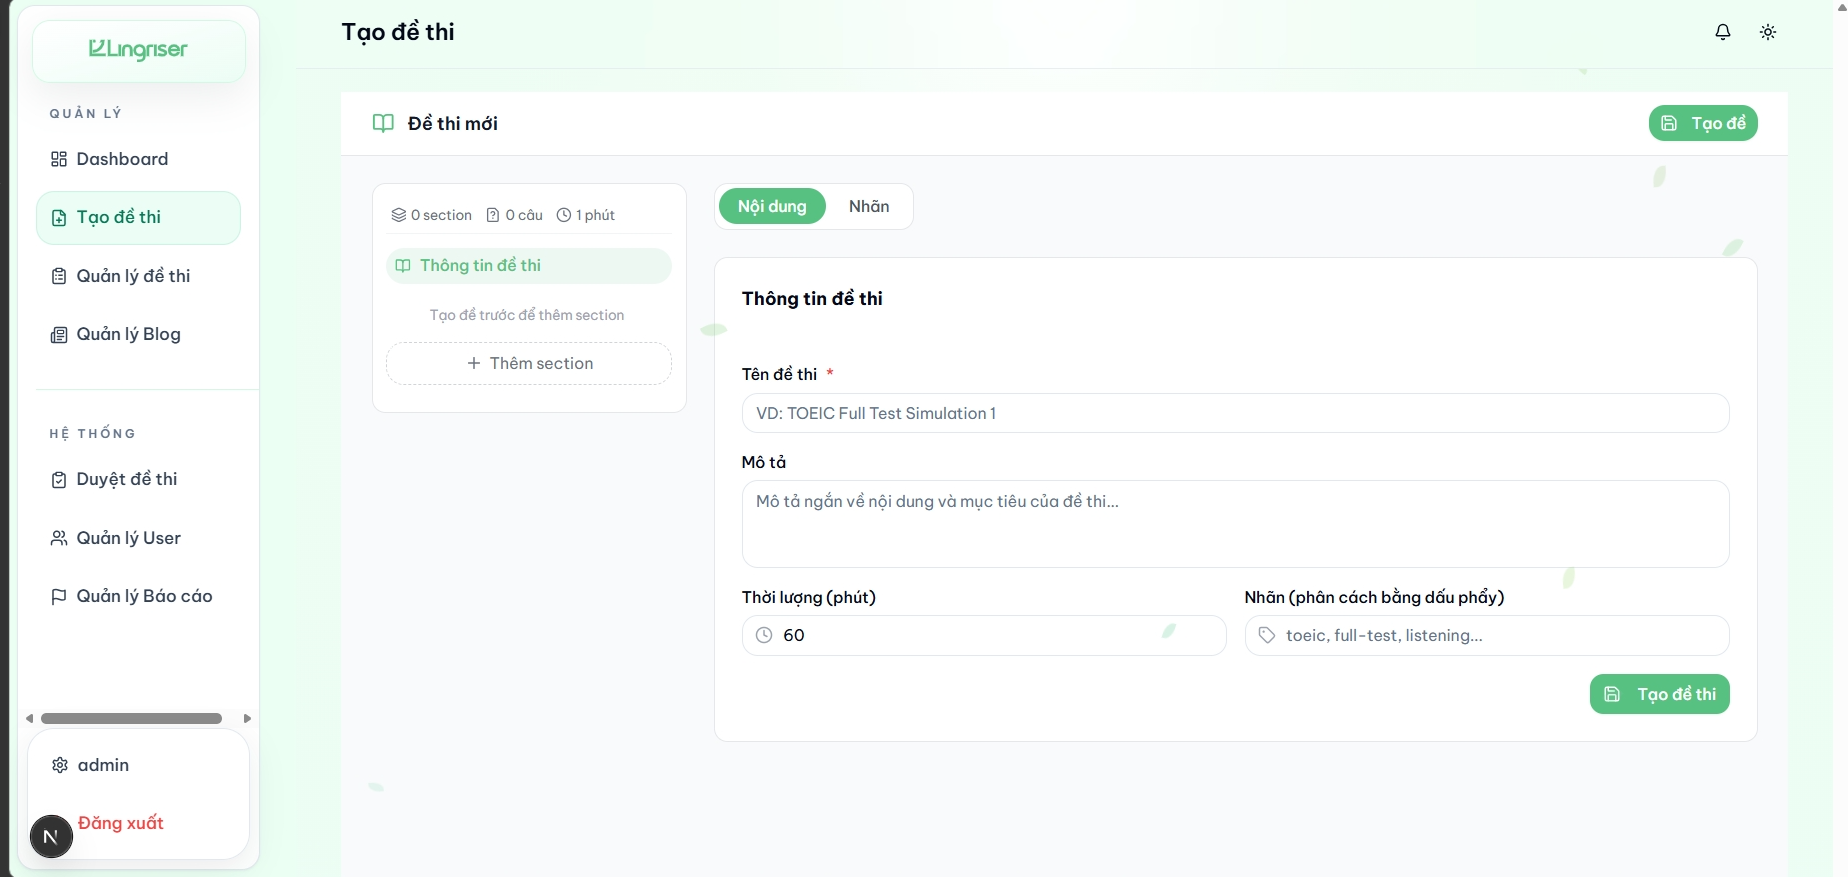
\includegraphics[width=0.75\linewidth]{graphics/ui/admin/exam-creation.jpg}%
    }{%
        \fbox{\parbox[c][0.3\textheight][c]{0.9\linewidth}{\centering Placeholder cho giao diện tạo đề thi\newline (chưa có tệp hình trong thư mục graphics/ui/admin)}}%
    }
    \captionsetup{skip=5pt}
    \caption{Giao diện tạo đề thi}
    \label{fig:admin-exam-creation}
\end{figure}

\noindent Giao diện tạo đề thi giúp quản trị viên nhập nhanh thông tin cho một đề mới. Bên trái là khu vực quản lý cấu trúc đề và thêm section, còn bên phải là biểu mẫu nhập tên đề, mô tả, thời lượng và nhãn phân loại. Các nút ``Tạo đề'' được đặt ở vị trí dễ thấy, giúp thao tác tạo đề diễn ra nhanh và rõ ràng hơn.



\subsubsection{Quản lý đề thi}

\begin{figure}[H]
    \centering
    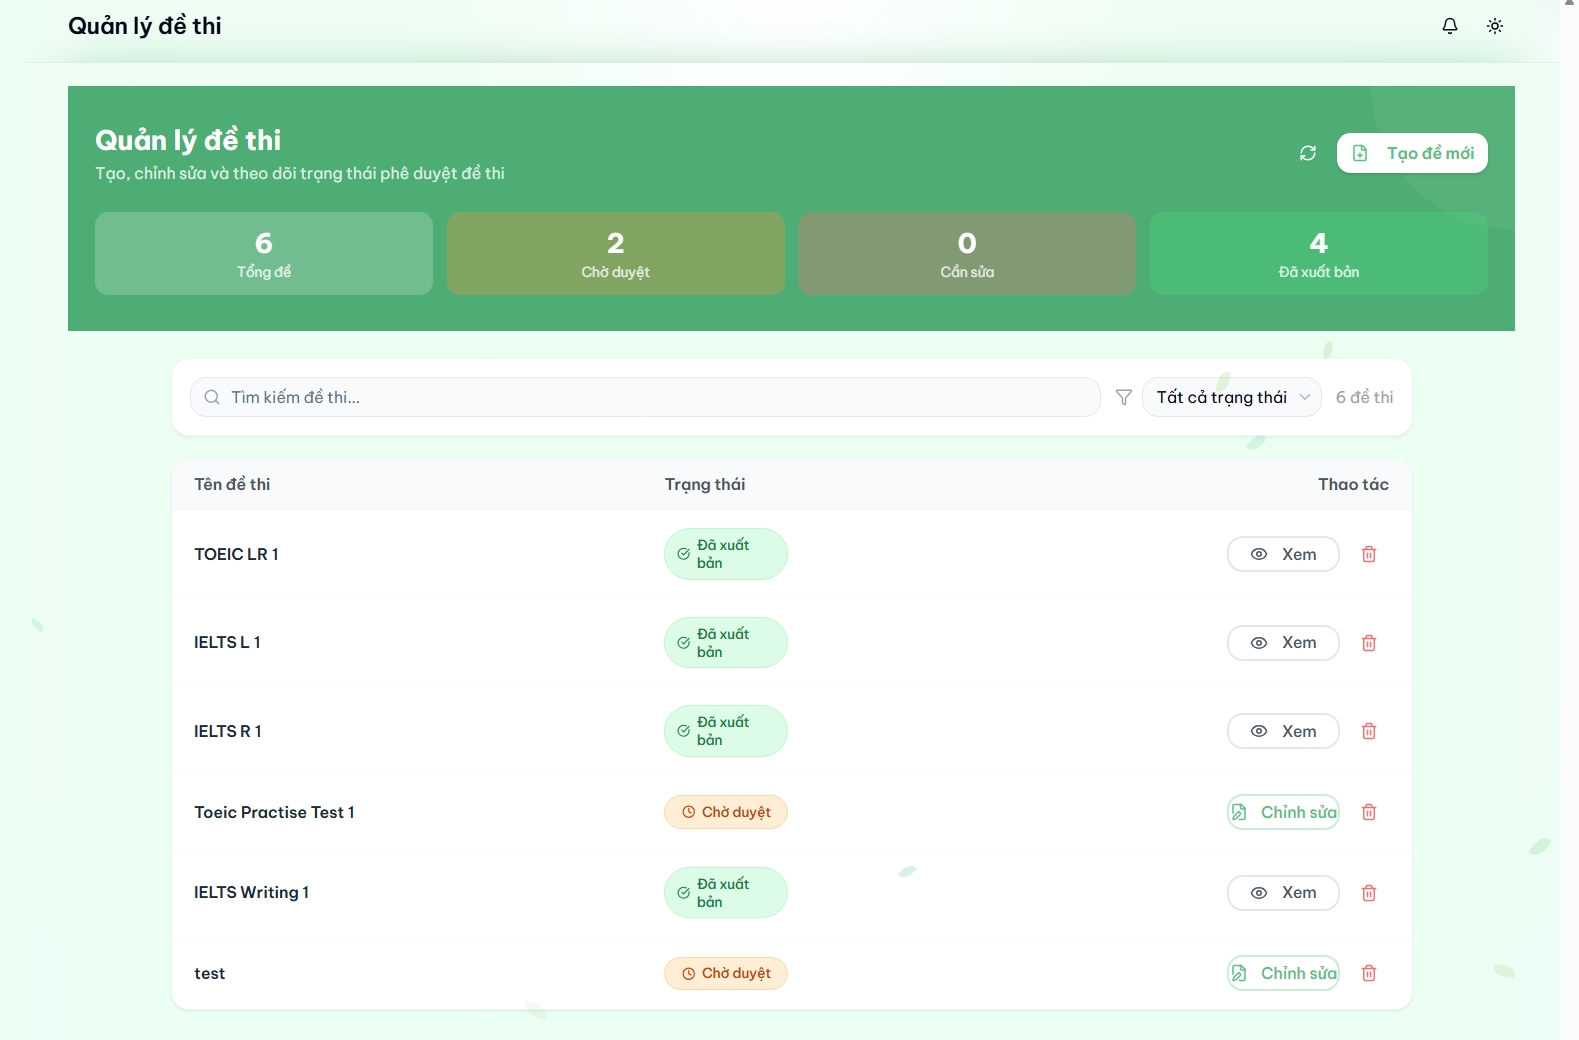
\includegraphics[width=0.75\linewidth]{graphics/ui/admin/exam-management.jpg}
    \captionsetup{skip=5pt}
    \caption{Giao diện quản lý đề thi}
    \label{fig:admin-exam-management}
\end{figure}

\noindent Trang quản lý đề thi giúp quản trị viên theo dõi và xử lý danh sách đề thi trong hệ thống. Phần đầu trang hiển thị nhanh số lượng đề theo từng trạng thái như tổng đề, chờ duyệt, cần sửa và đã xuất bản. Bên dưới là khu vực tìm kiếm, lọc trạng thái và bảng danh sách đề thi, trong đó mỗi dòng cho biết tên đề, trạng thái hiện tại và các nút thao tác như xem hoặc chỉnh sửa. Cách bố trí này giúp việc quản lý đề thi hằng ngày trở nên rõ ràng và thuận tiện hơn.




\subsubsection{Quản lý bài viết}

\begin{figure}[H]
    \centering
    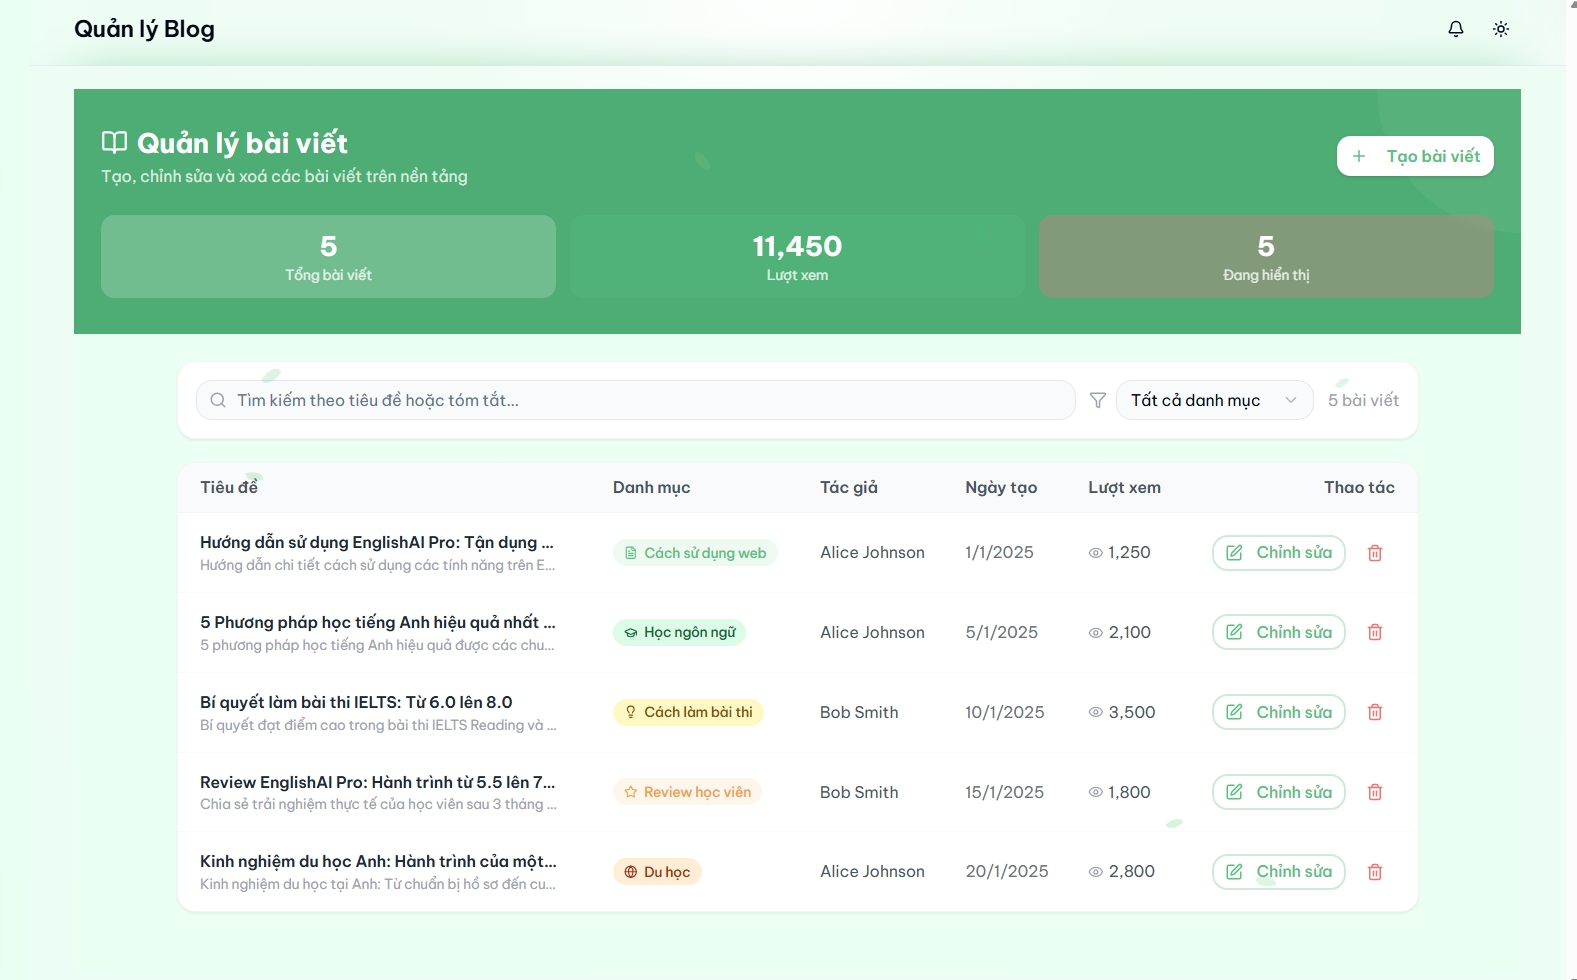
\includegraphics[width=0.75\linewidth]{graphics/ui/admin/blog-management.jpg}
    \captionsetup{skip=5pt}
    \caption{Giao diện quản lý bài viết blog}
    \label{fig:admin-blog-management}
\end{figure}

\noindent Giao diện quản lý blog được thiết kế rõ ràng để hỗ trợ quản trị viên theo dõi và điều phối nội dung trên hệ thống. Phần đầu trang hiển thị tiêu đề khu vực cùng các chỉ số tổng quan, giúp người dùng nắm nhanh số lượng bài viết hoặc trạng thái hiện tại. Bên dưới là thanh tìm kiếm, bộ lọc và danh sách bài viết được trình bày theo từng thẻ hoặc dòng, trong đó mỗi mục thể hiện các thông tin quan trọng như tiêu đề, thời gian cập nhật và trạng thái hiển thị. Nhờ cách bố trí này, việc tìm kiếm, kiểm tra và quản lý nội dung blog trở nên thuận tiện, trực quan và tiết kiệm thời gian hơn.

\subsubsection{Phê duyệt đề thi}

\begin{figure}[H]
    \centering
    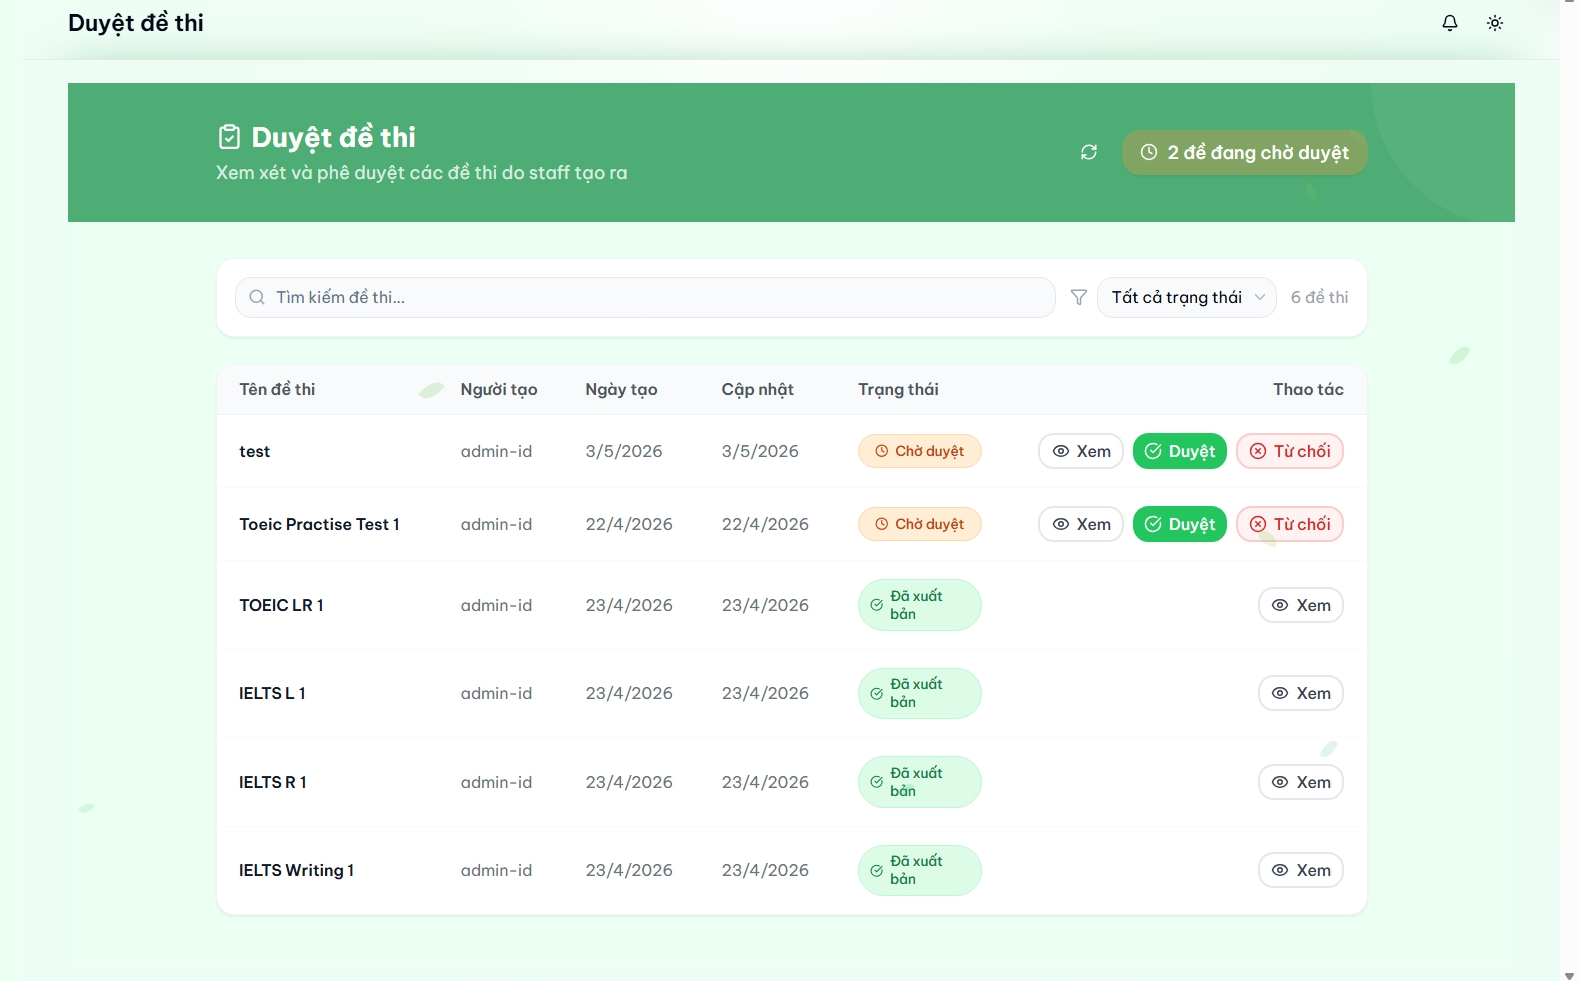
\includegraphics[width=0.75\linewidth]{graphics/ui/admin/exam-approval.jpg}
    \captionsetup{skip=5pt}
    \caption{Giao diện duyệt đề thi}
    \label{fig:admin-exam-approval}
\end{figure}

\noindent Trang duyệt đề thi giúp quản trị viên kiểm tra và xử lý các đề đang chờ phê duyệt. Phần đầu trang hiển thị số lượng đề chờ duyệt, đi kèm ô tìm kiếm và bộ lọc trạng thái để tìm đề nhanh hơn. Bên dưới là bảng danh sách đề thi với các thông tin như tên đề, người tạo, ngày tạo, trạng thái và các nút thao tác như xem, duyệt hoặc từ chối. Cách trình bày này giúp quá trình kiểm duyệt diễn ra rõ ràng và thuận tiện hơn.

\subsubsection{Quản lý người dùng}

\begin{figure}[H]
    \centering
    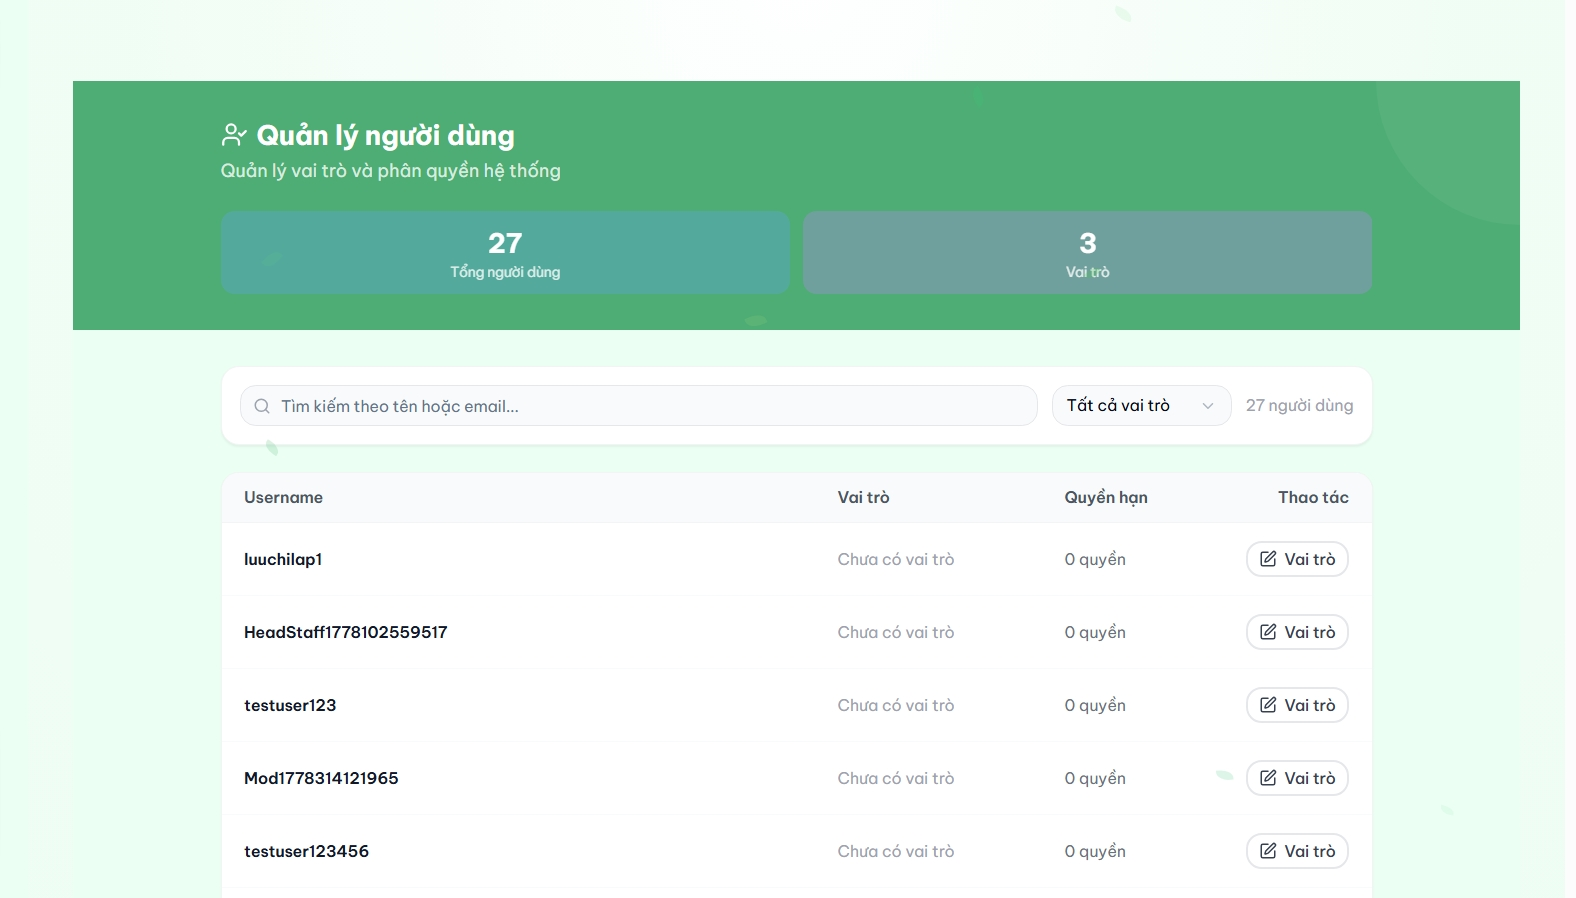
\includegraphics[width=0.75\linewidth]{graphics/ui/admin/user-management.jpg}
    \captionsetup{skip=5pt}
    \caption{Giao diện quản lý người dùng}
    \label{fig:admin-user-management}
\end{figure}

\noindent Giao diện quản lý người dùng được thiết kế rõ ràng để hỗ trợ quản trị viên theo dõi và kiểm soát tài khoản trong hệ thống. Phần đầu trang thường hiển thị tiêu đề khu vực, thanh tìm kiếm và các bộ lọc theo vai trò hoặc trạng thái, giúp việc tra cứu trở nên nhanh chóng hơn. Bên dưới là danh sách người dùng với những thông tin quan trọng như tên, email, vai trò và trạng thái tài khoản, đi kèm các thao tác quản trị cần thiết. Cách bố trí này giúp việc quản lý người dùng diễn ra trực quan, thuận tiện và phù hợp với nhu cầu vận hành hằng ngày.


\subsubsection{Quản lý báo cáo}

\begin{figure}[H]
    \centering
    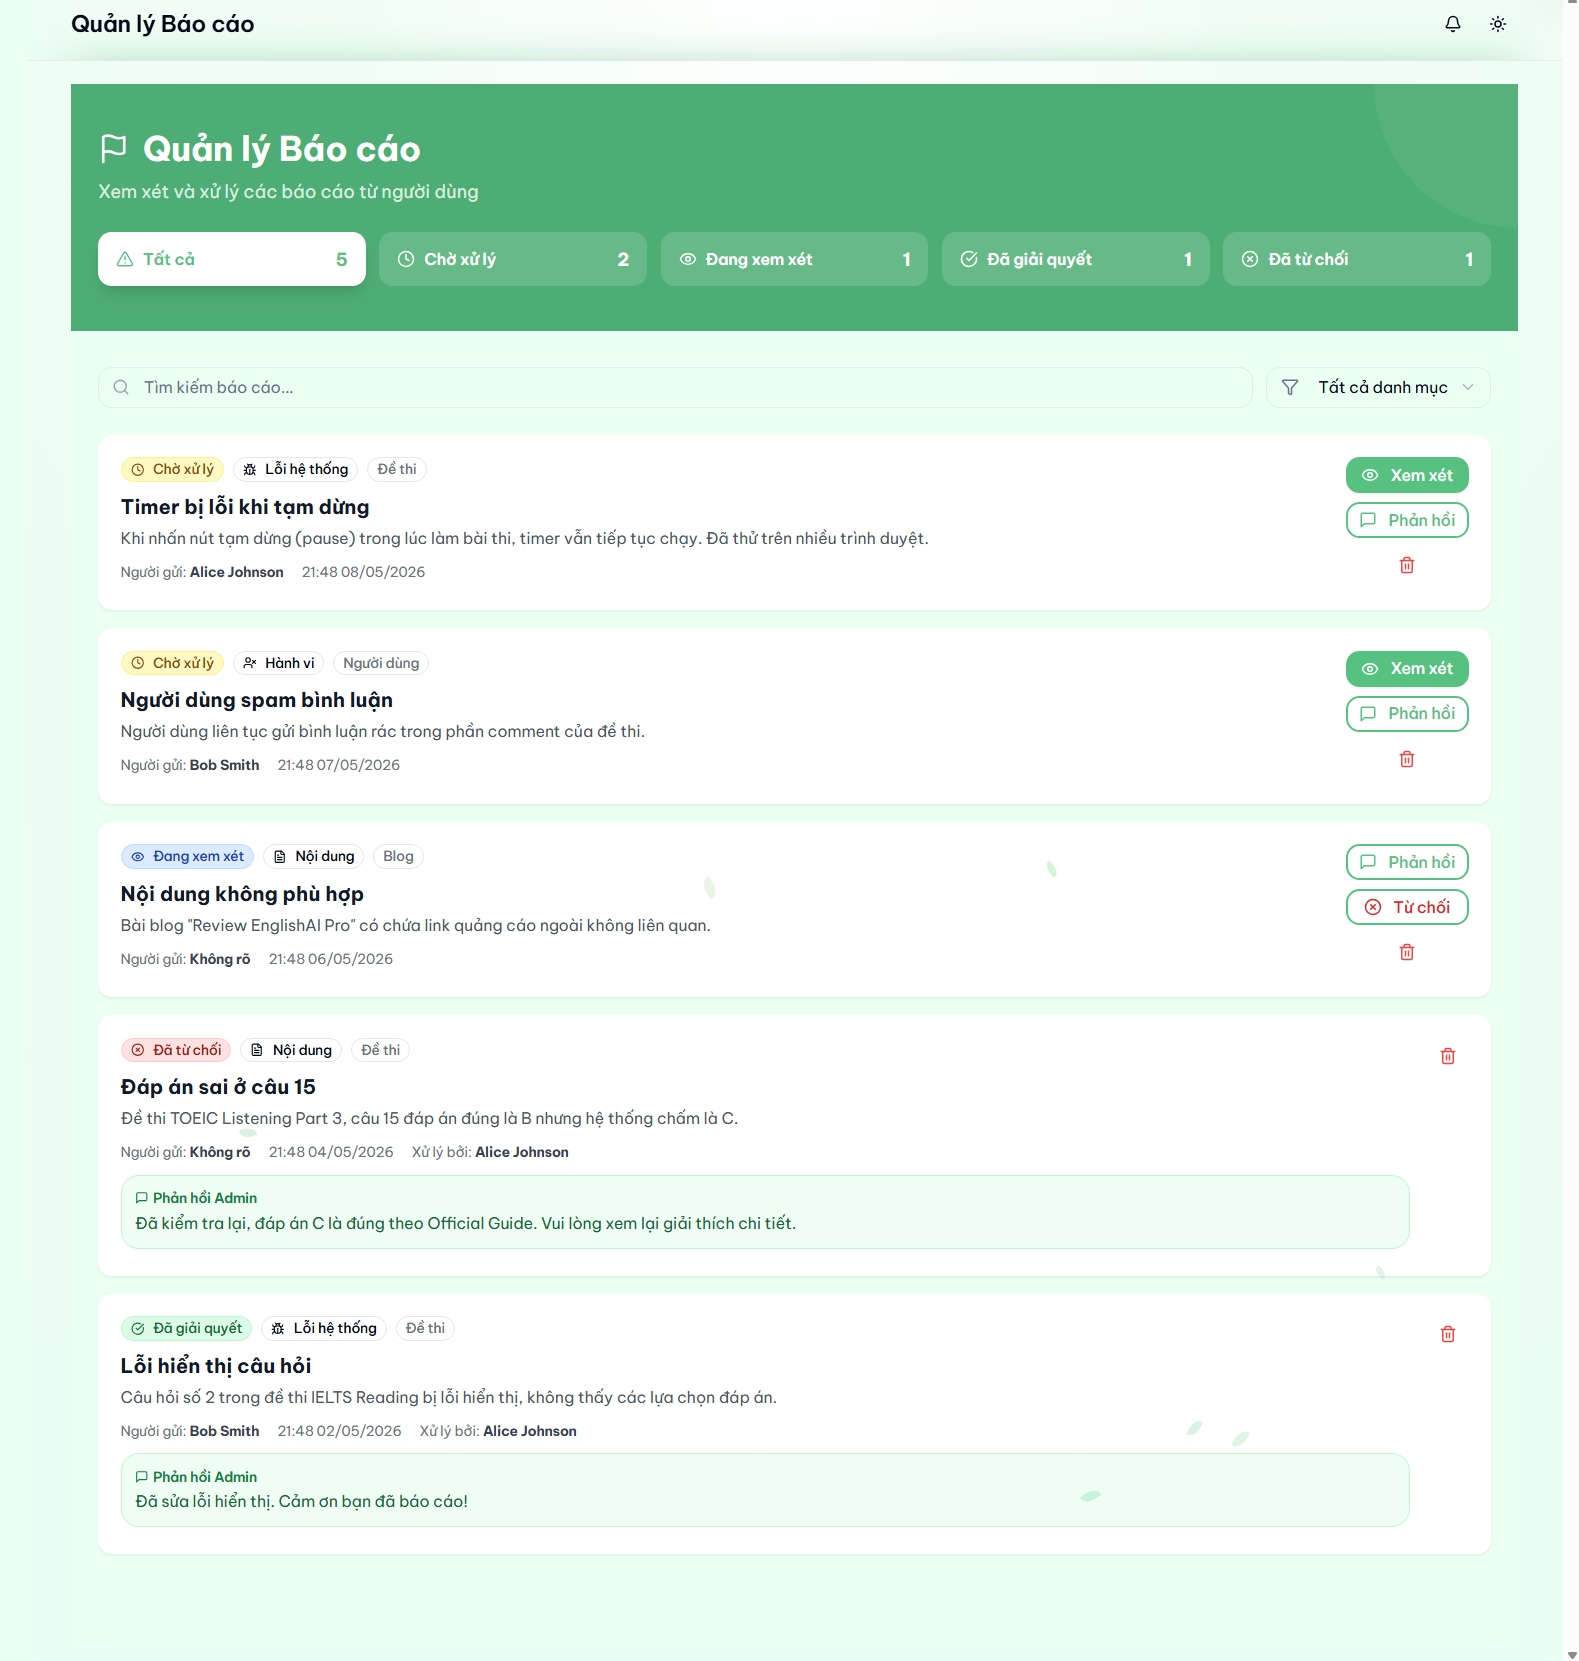
\includegraphics[width=0.75\linewidth]{graphics/ui/admin/norify-management.jpg}
    \captionsetup{skip=5pt}
    \caption{Giao diện quản lý báo cáo}
    \label{fig:admin-report-management}
\end{figure}

\noindent Giao diện quản lý báo cáo được trình bày rõ ràng để hỗ trợ quản trị viên tiếp nhận và xử lý phản ánh từ người dùng. Phần đầu trang nổi bật với tiêu đề khu vực, các thẻ thống kê theo trạng thái như chờ xử lý, đang xem xét, đã giải quyết hoặc đã từ chối, giúp người quản trị nắm nhanh tình hình chung. Bên dưới là thanh tìm kiếm, bộ lọc danh mục và danh sách báo cáo được hiển thị theo từng thẻ nội dung, trong đó mỗi báo cáo cho biết tiêu đề, loại vấn đề, người gửi, thời gian tạo và các nút thao tác như xem xét, phản hồi hoặc từ chối. Cách bố trí này giúp quá trình rà soát báo cáo diễn ra mạch lạc, trực quan và thuận tiện hơn trong vận hành hằng ngày.


\subsection{Trang chủ luyện nói}

Phần này trình bày các giao diện tiêu biểu của \textit{LingriserSpeaking}, mô-đun luyện nói tiếng Anh tích hợp AI được phát triển song song với nền tảng chính. Khác với nhóm wireframe trước đó vốn tập trung vào hệ thống luyện thi IELTS và TOEIC tổng quát, các màn hình trong LingriserSpeaking được tổ chức xoay quanh chu trình học tập theo tuần, phối hợp giữa học sinh, phụ huynh, mentor và quản trị viên. Các giao diện dưới đây cho thấy cách hệ thống hỗ trợ từ giai đoạn định hướng chương trình, luyện nói với AI, đặt lịch học đồng bộ cho đến theo dõi tiến độ và vận hành toàn bộ nền tảng.



\subsection{Bảng điều khiển người học}

\begin{figure}[H]
    \centering
    
\includegraphics[width=0.75\linewidth]{graphics/lingriser/dashboard.png}
    \captionsetup{skip=5pt}
    \caption{Bảng điều khiển học sinh trong Lingriser Speaking}
    \label{fig:lingriser-student-dashboard}
\end{figure}
\noindent Dashboard học sinh là điểm điều phối trung tâm của toàn bộ trải nghiệm luyện nói trên LingriserSpeaking. Bố cục của màn hình ưu tiên việc tóm tắt nhanh module hiện tại, các buổi học sắp tới, mức độ luyện tập với AI và tiến trình của chương trình học theo tuần. Các khối nội dung được sắp xếp theo hướng giúp người học nhìn thấy ngay mình đang ở đâu trong lộ trình, cần hoàn thành hoạt động nào tiếp theo và đâu là những dữ liệu quan trọng như video tiến độ hoặc lịch học đồng bộ. Nhờ đó, dashboard không chỉ đóng vai trò hiển thị thông tin mà còn trở thành điểm xuất phát tự nhiên cho các phiên luyện nói hằng ngày.

\subsection{Đặt lịch gia sư}

\begin{figure}[H]
    \centering
    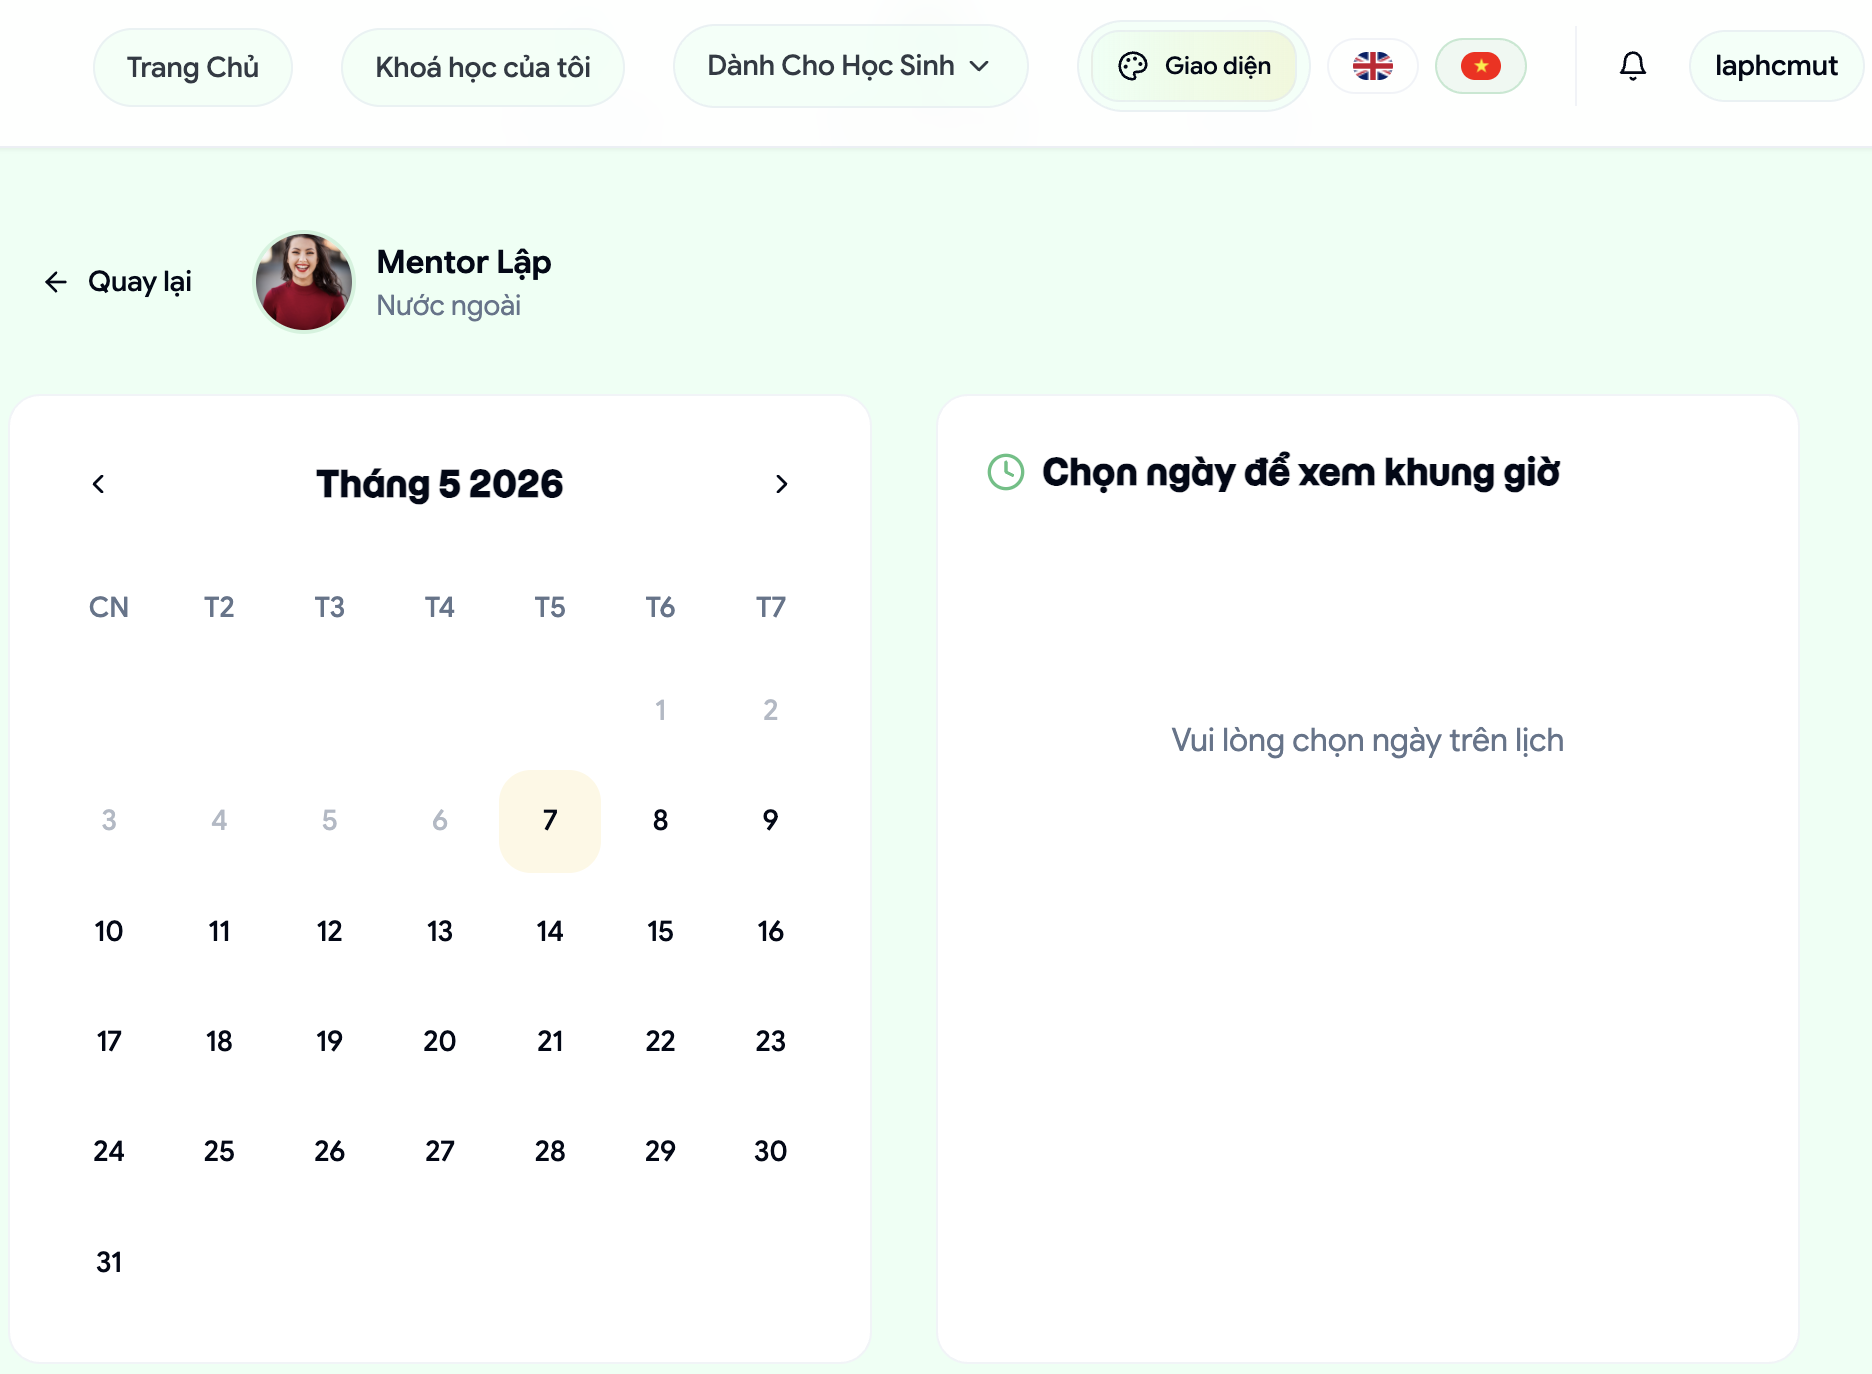
\includegraphics[width=0.9\linewidth]{graphics/lingriser/mentor.png}
    \captionsetup{skip=5pt}
    \caption{Giao diện lựa chọn mentor và đặt lịch video call}
    \label{fig:lingriser-mentor-booking}
\end{figure}
\noindent Giao diện làm việc với mentor tập trung vào hai nhu cầu chính: lựa chọn người hướng dẫn phù hợp và chốt lịch học vào các khung giờ khả dụng. Màn hình kết hợp phần thông tin hồ sơ mentor với khu vực lịch hoặc các phiên học để người dùng có thể so sánh, theo dõi tình trạng trống và thực hiện đặt lịch ngay trong cùng một luồng thao tác. Cách tổ chức này làm giảm độ phân mảnh của trải nghiệm, giúp việc chuyển từ luyện nói bất đồng bộ với AI sang buổi học đồng bộ với người thật diễn ra mạch lạc hơn. Đồng thời, giao diện cũng góp phần làm rõ vai trò của mentor như một tác nhân tiếp nối trực tiếp kết quả luyện tập trong tuần.

\subsection{Bảng điều khiển phụ huynh}

\begin{figure}[H]
    \centering
    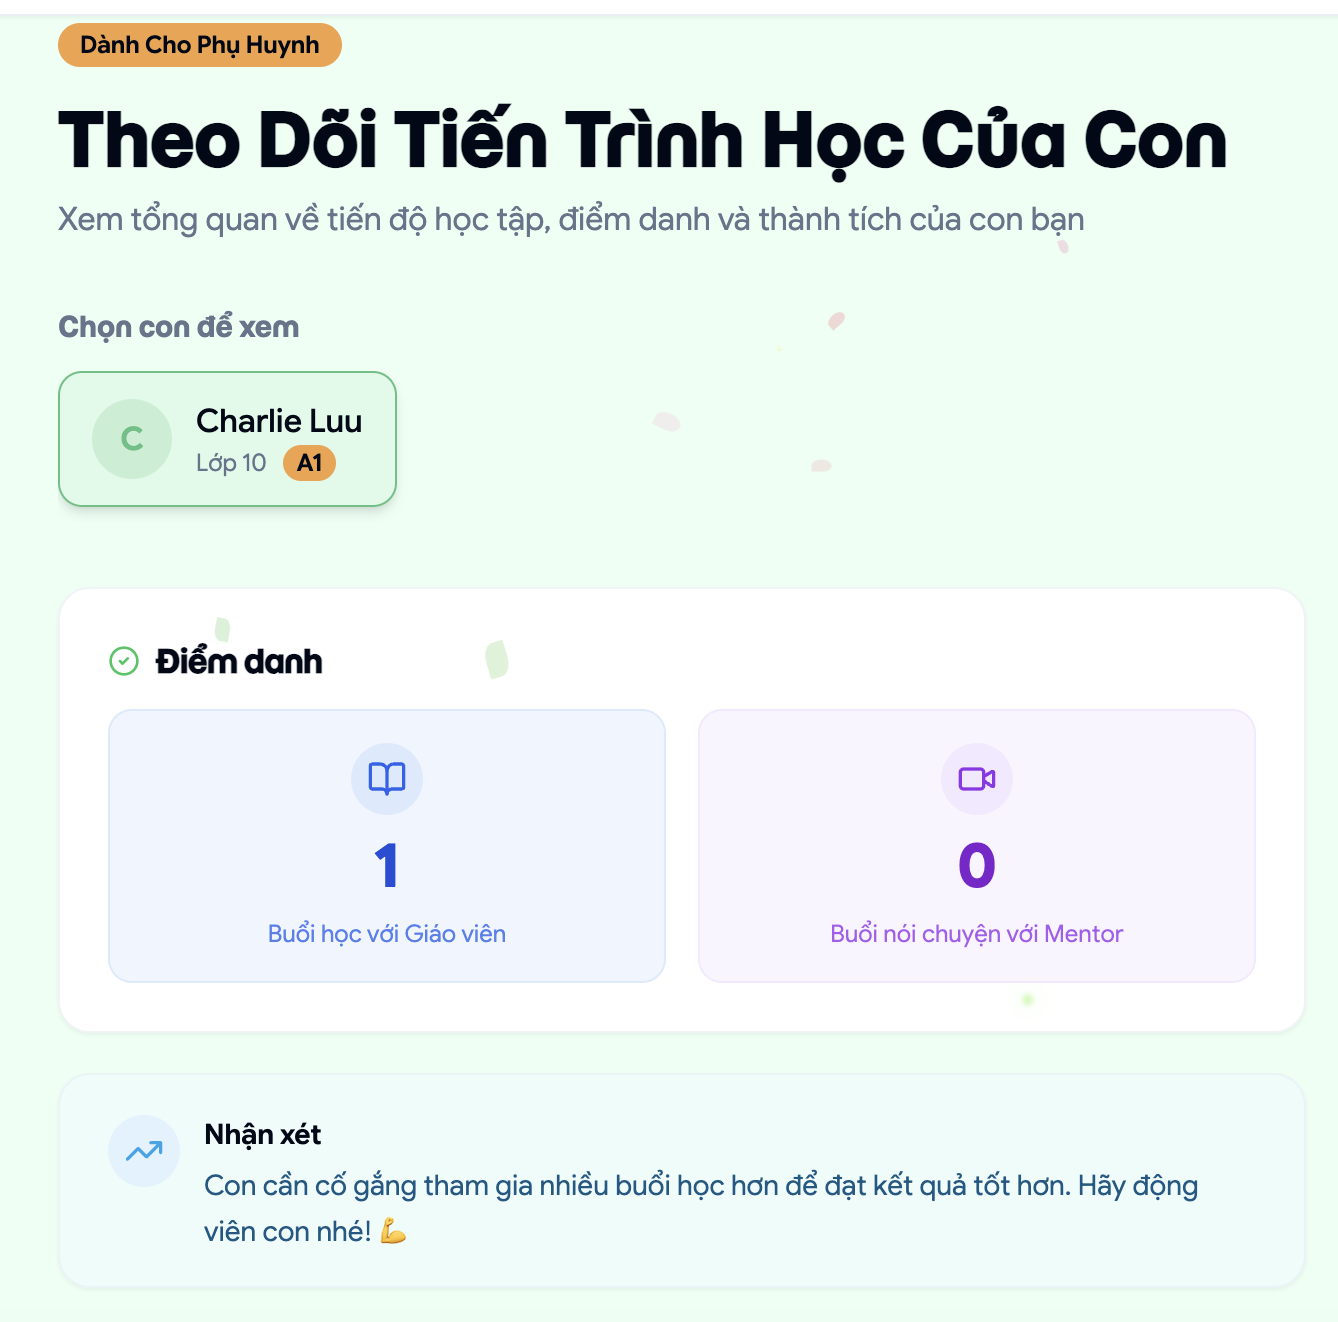
\includegraphics[width=0.88\linewidth]{graphics/lingriser/parents.png}
    \captionsetup{skip=5pt}
    \caption{Bảng điều khiển phụ huynh theo dõi tiến trình học tập}
    \label{fig:lingriser-parent-dashboard}
\end{figure}
\noindent Dashboard phụ huynh được thiết kế như một không gian quan sát tiến trình học tập của con thay vì một khu vực thao tác học trực tiếp. Giao diện ưu tiên các thành phần tổng hợp như thông tin học sinh, mức độ tham gia, lịch học, hoạt động gần đây và các chỉ báo tiến bộ để phụ huynh có thể nhanh chóng nắm bắt tình hình chung. Việc đưa dữ liệu AI practice, lịch sử học tập và video tiến độ vào cùng một màn hình giúp phụ huynh theo dõi sự thay đổi của người học theo thời gian mà không cần truy cập vào nhiều trang riêng lẻ. Đây là một điểm khác biệt quan trọng của LingriserSpeaking khi mở rộng giá trị của dữ liệu luyện nói sang cả bối cảnh đồng hành từ gia đình.

\subsection{Chương trình học}

\begin{figure}[H]
    \centering
    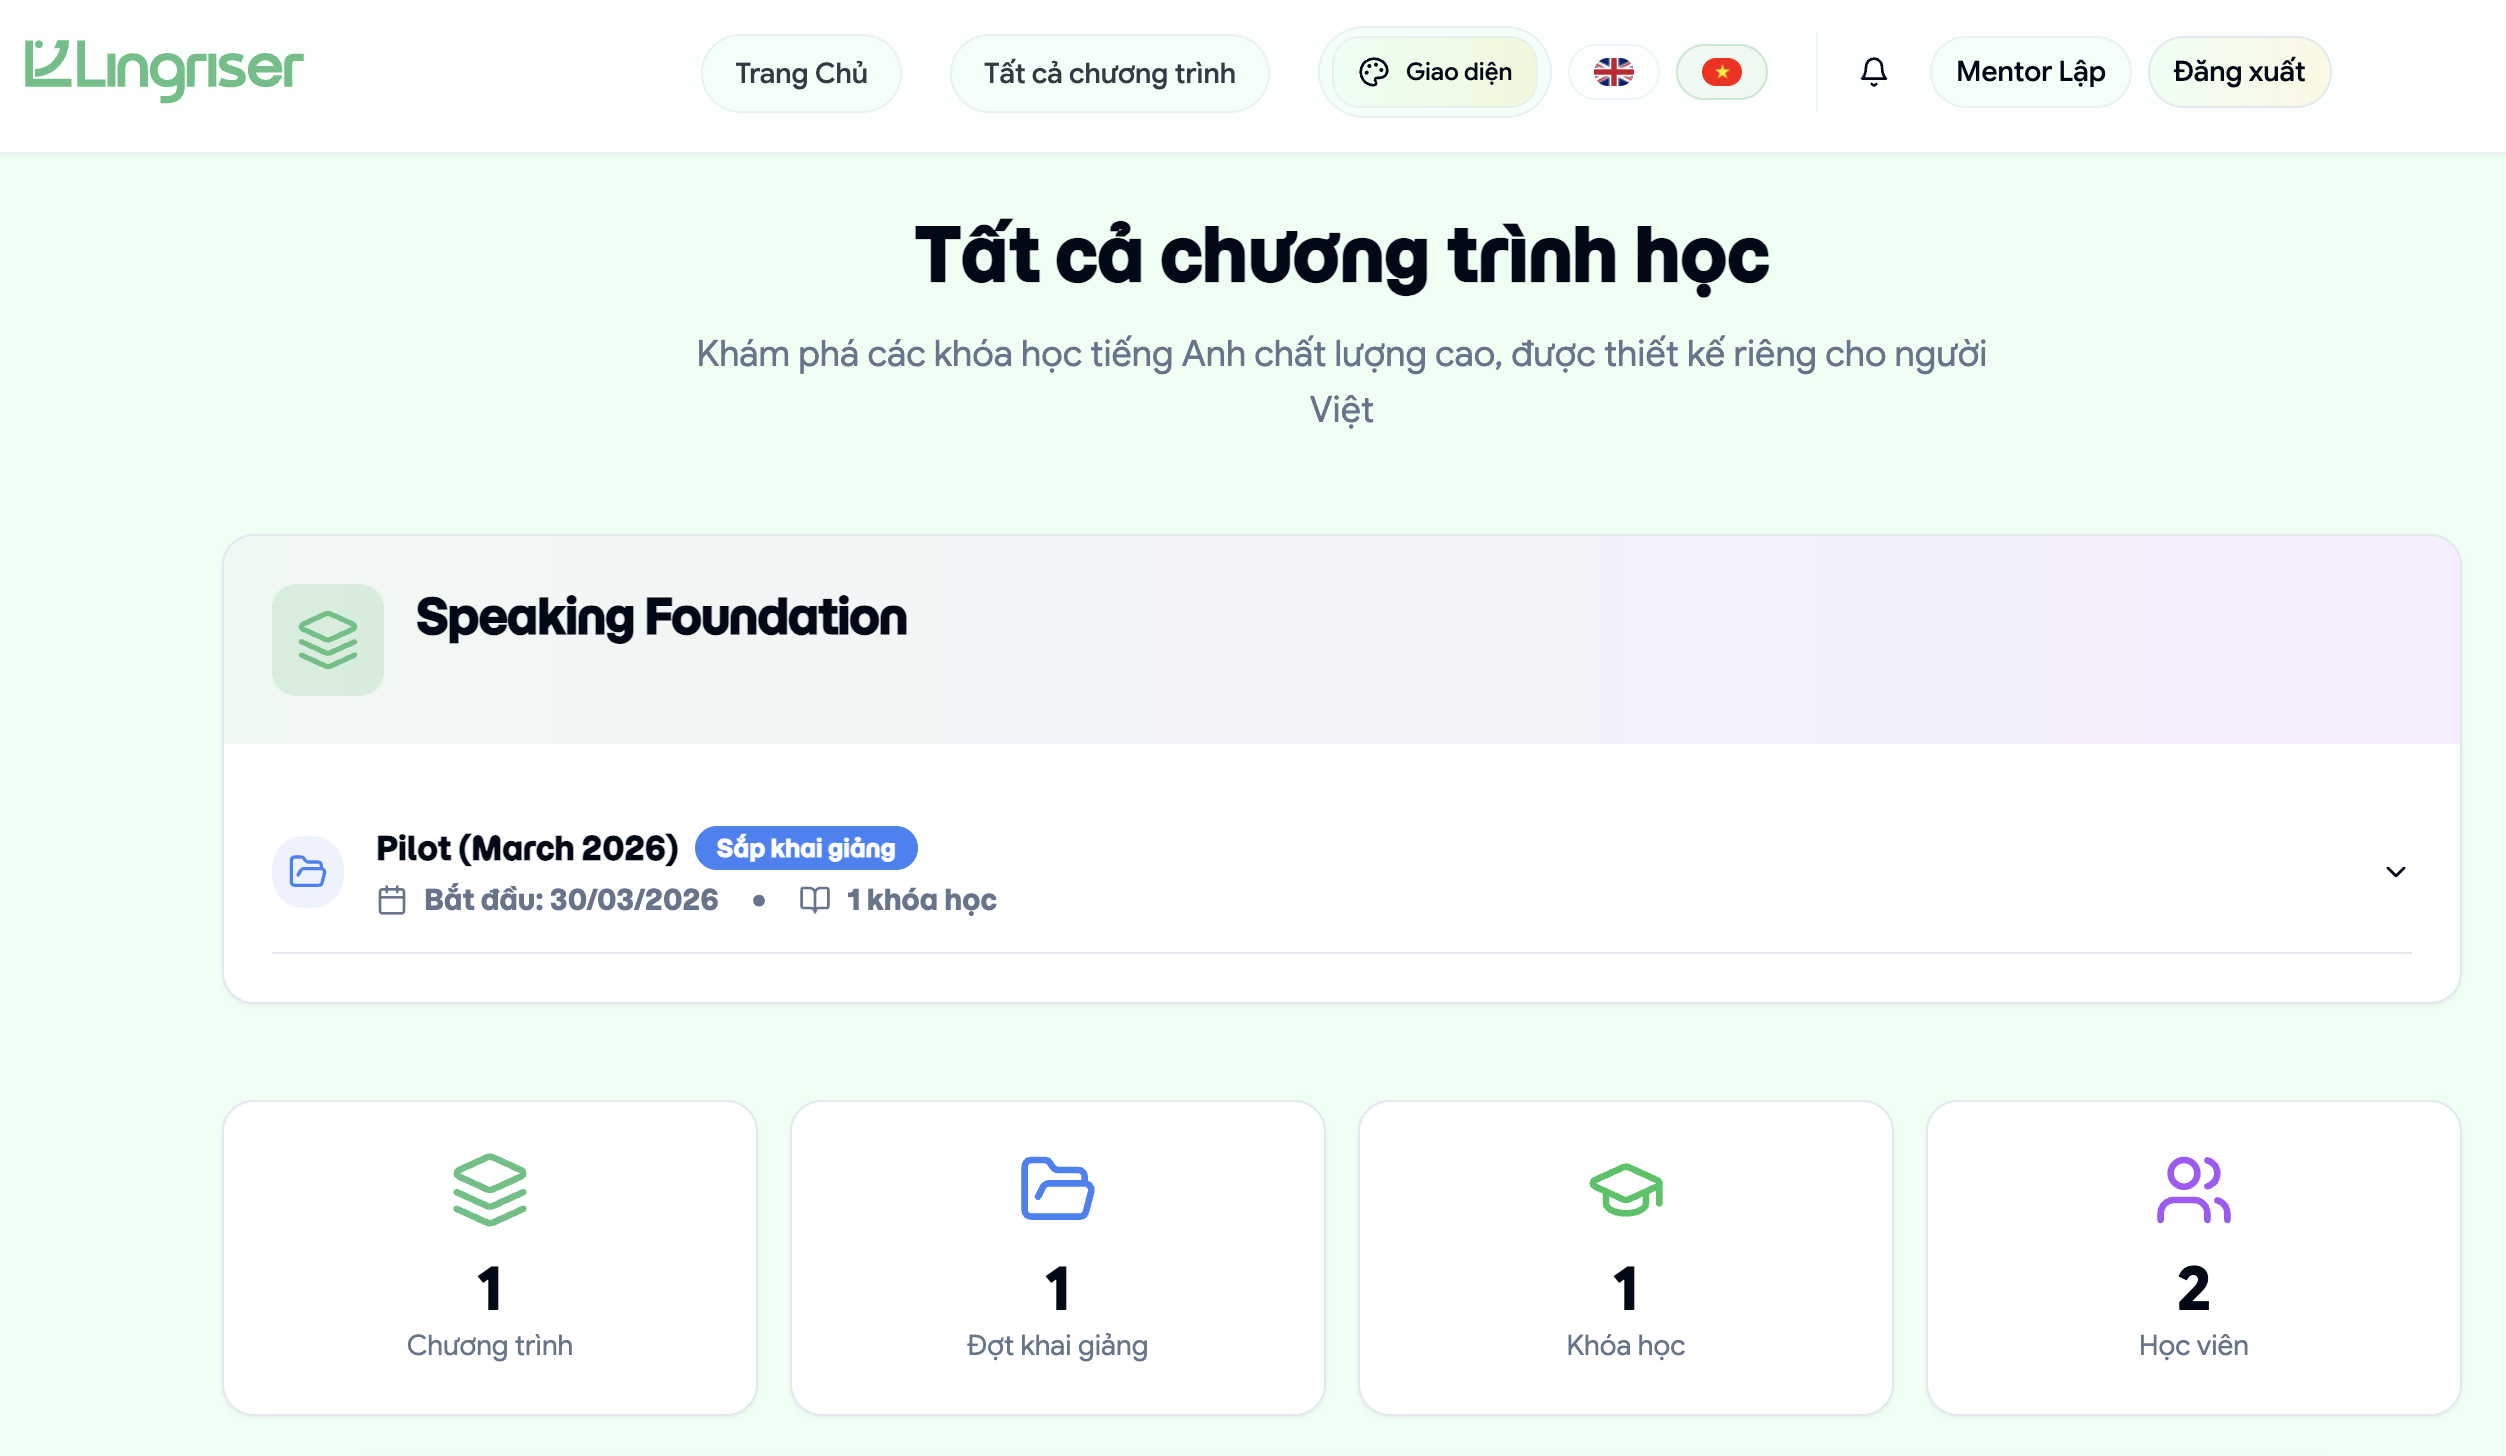
\includegraphics[width=0.9\linewidth]{graphics/lingriser/programs.png}
    \captionsetup{skip=5pt}
    \caption{Giao diện quản lý chương trình học và tiến trình theo mô-đun}
    \label{fig:lingriser-programs}
\end{figure}
\noindent Trang chương trình học trình bày cấu trúc đào tạo của LingriserSpeaking theo hướng phân cấp rõ ràng giữa chương trình, nhóm học, khóa học và các mô-đun. Nhờ cách bố trí này, người dùng hoặc quản trị viên có thể theo dõi được mối quan hệ giữa nội dung học, tiến độ mở khóa và trạng thái tham gia của từng học viên. Giao diện không chỉ hỗ trợ quan sát tổng thể mà còn giúp định vị chính xác vị trí của người học trong lộ trình 8 tuần, từ đó tạo nền tảng cho việc gắn mục tiêu tuần, đặt lịch với mentor và lưu lịch sử luyện tập theo từng giai đoạn. Về mặt thiết kế thông tin, đây là màn hình giữ vai trò liên kết giữa cấu trúc học thuật và các hoạt động Speaking diễn ra hằng ngày.

\subsection{Bảng điều khiển quản trị}

\begin{figure}[H]
    \centering
    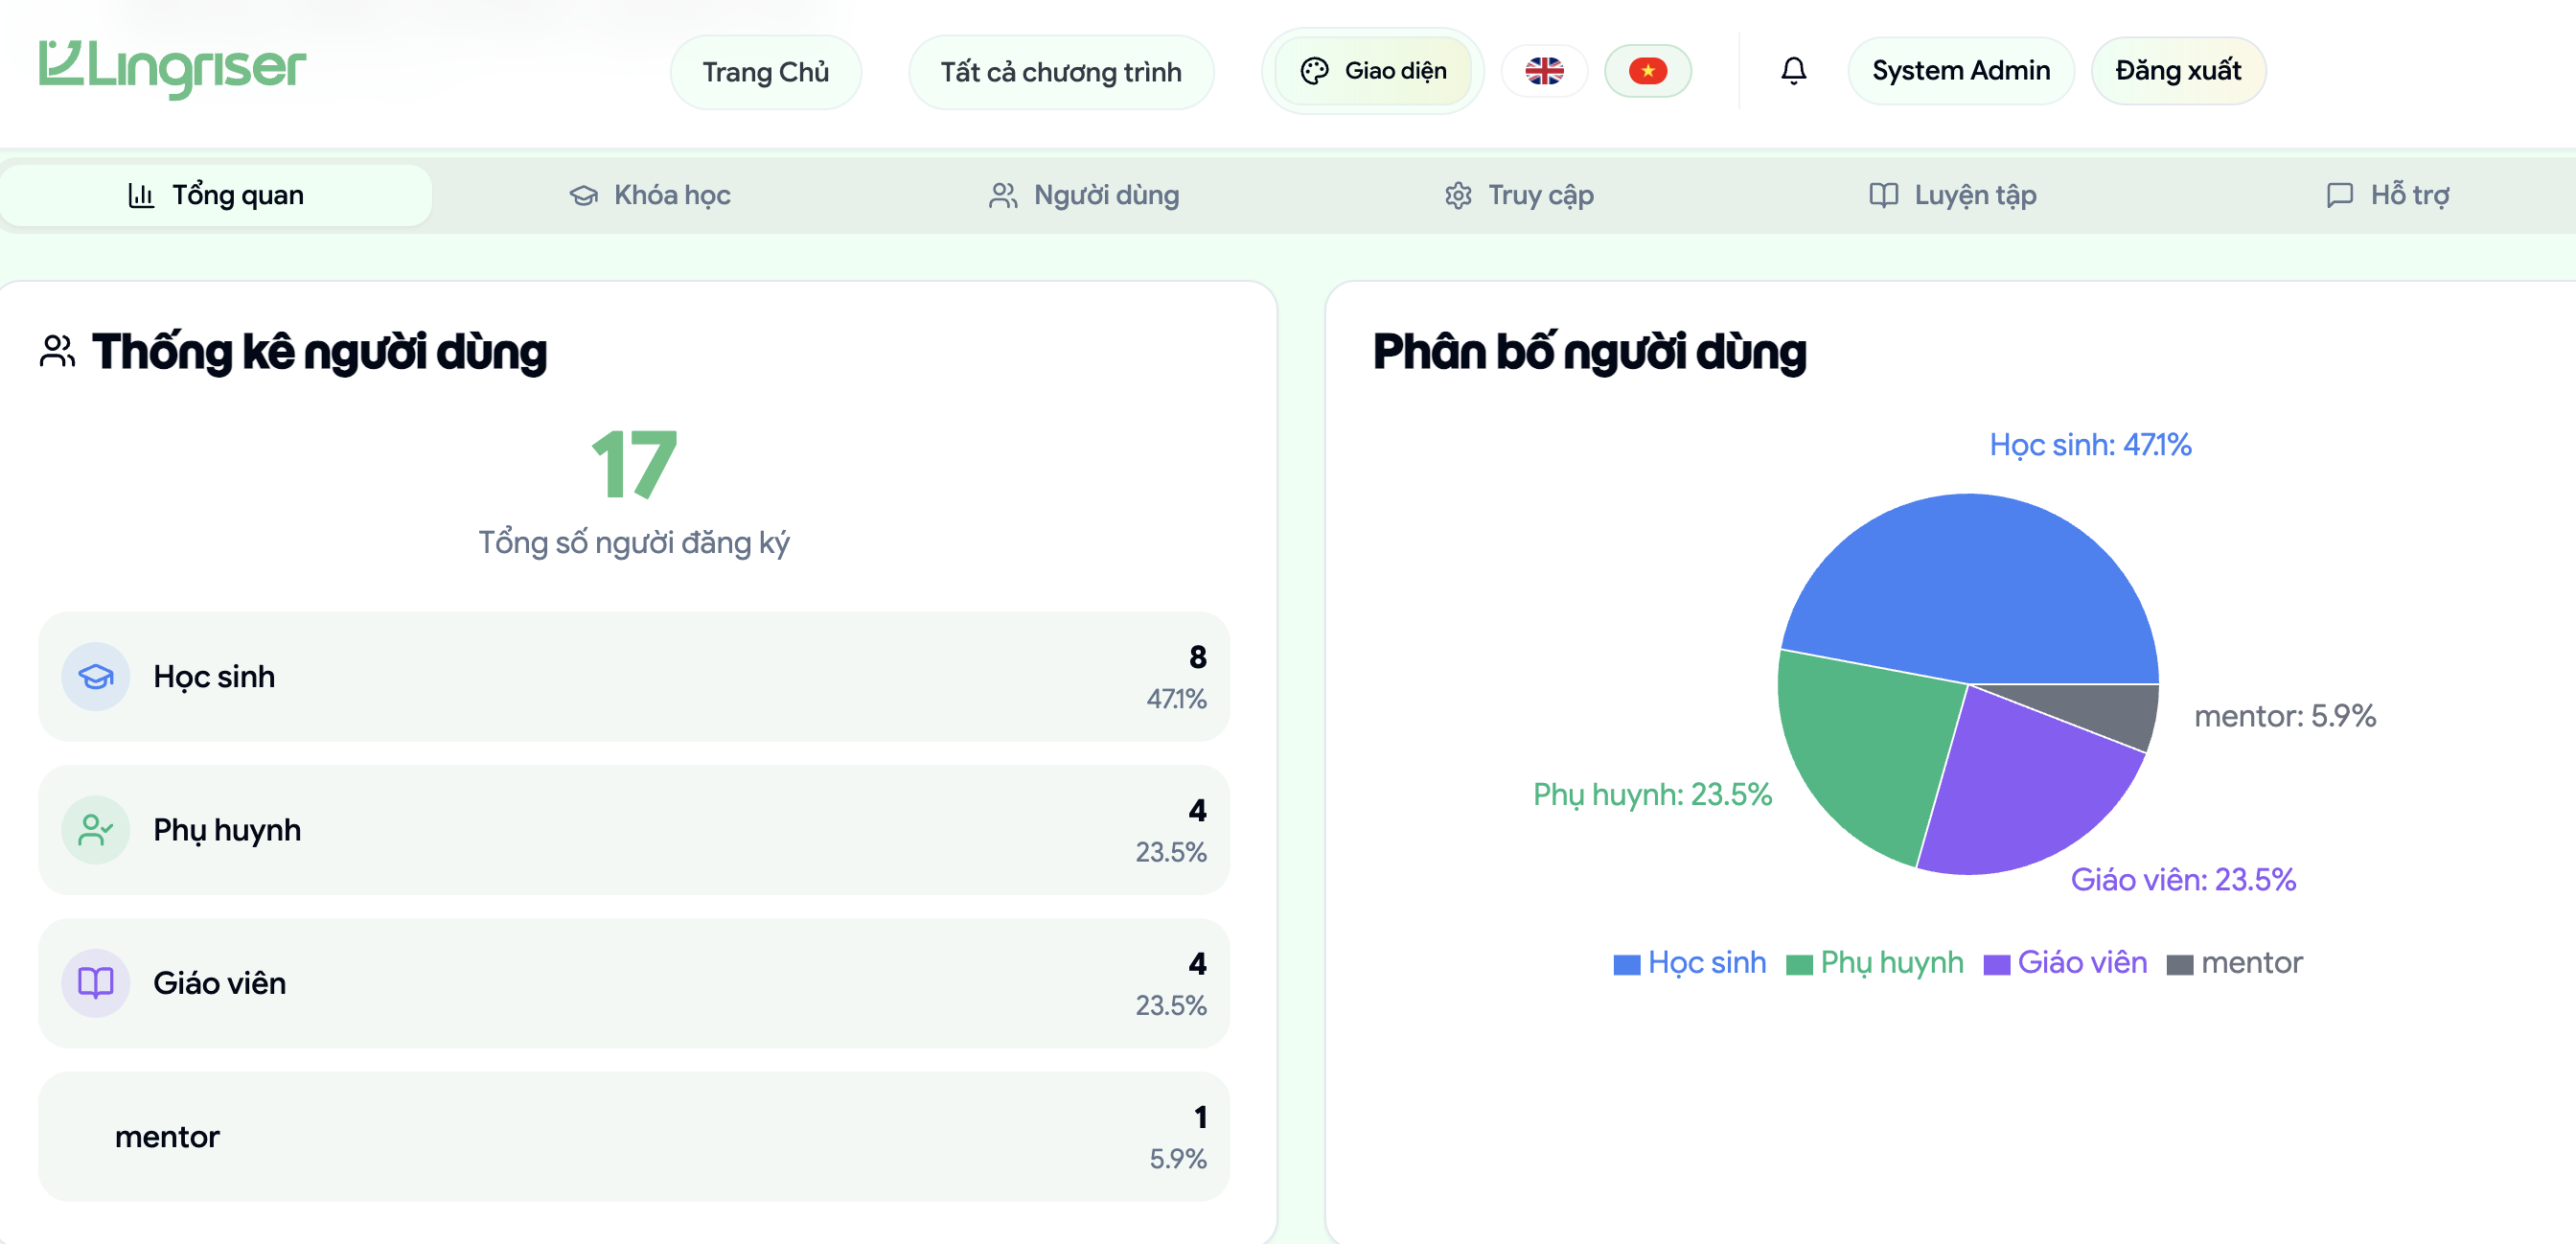
\includegraphics[width=0.75\linewidth]{graphics/lingriser/admin.png}
    \captionsetup{skip=5pt}
    \caption{Bảng điều khiển quản trị của LingriserSpeaking}
    \label{fig:lingriser-admin-dashboard}
\end{figure}
\noindent Bảng điều khiển quản trị là khu vực vận hành toàn bộ hệ sinh thái LingriserSpeaking ở cấp độ hệ thống. Bố cục của màn hình nhấn mạnh các khối thống kê tổng quan kết hợp với các khu vực chuyên trách như quản lý người dùng, quản lý khóa học, theo dõi lượt truy cập, thống kê số phiên luyện tập và hỗ trợ hội thoại với người dùng. Cách tổ chức này cho phép quản trị viên vừa có cái nhìn khái quát về trạng thái nền tảng, vừa nhanh chóng đi sâu vào từng nhóm tác vụ vận hành cụ thể. Trong bối cảnh một nền tảng học tập có nhiều vai trò tương tác như LingriserSpeaking, giao diện admin đóng vai trò quan trọng trong việc duy trì tính ổn định, khả năng kiểm soát dữ liệu và chất lượng dịch vụ.


\section{Kết luận chương}
Chương này đã trình bày hệ thống wireframe cho các màn hình cốt lõi của nền tảng luyện thi tích hợp AI, từ các giao diện hướng đến người học cho đến các công cụ quản trị nội dung. Thông qua việc mô tả mục tiêu, bố cục và luồng tương tác của từng màn hình, chương đã làm rõ cách hệ thống hỗ trợ người dùng trong toàn bộ hành trình học tập: từ tiếp cận nền tảng, đăng nhập, lựa chọn bài luyện, làm bài, nhận phản hồi, tích lũy kiến thức đến theo dõi tiến độ cá nhân. Đây là cơ sở quan trọng để triển khai giao diện chi tiết, kiểm thử trải nghiệm người dùng và hiện thực hóa hệ thống trong các giai đoạn tiếp theo.